  \chapter{Lokale Flächentheorie im euklidischen Raum}
\section{Grundbegriffe der Flächentheorie}
\setcounter{subsection}{-1}
\subsection{$p$-dimensionale Flächen im affinen $\IR^n$}
Sei \(1 < p < n\) fest gewählt (in Anwendungen meist \(p = 2, n= 3\)).
 
\begin{definition}[Parametrisierte \(\C^r\)-\(p\)-Fläche (\(r \ge 0\))]\index{Fläche}
\(\C^r\)-Abbildung \(x\colon G \subset \IR^p \to \IR^n\)
\[
 u = \left( u^1, \dots , u^p \right) \mapsto x(u) = \left(x^1(u), \dots, x^n (u) \right) 
\]
wobei \(G\) ein \uline{Gebiet} des \(\IR^p\) (d.h. offen und zusammenhängend) ist.\\
\uline{Parameter:}\index{Fläche!Parameter} \[ u^1, \dots , u^p \quad \text{bei }n = 3\text{ meist }(u,v) \]
\uline{Parameterlinien:}\index{Fläche!Parameterlinie}
\[u^\varrho \mapsto x \left(u^1_0, \dots , u^\varrho , \dots , u^p_0 \right)\]
\uline{Spur:}\index{Fläche!Spur} \[M:= x\left[G \right] \subset \IR^n\]
\uline{Regularität \(r \geq 1\)}\index{Fläche!regulär}: Die partiellen Ableitungen 
\[x_\varrho := \partial_\varrho x = \frac{\partial x}{\partial u^\varrho} \quad (\varrho = 1, \dots , p)\] 
sind überall linear unabhängig (sonst \uline{Singularitäten})\index{Fläche!Singularität}.
\end{definition}

\begin{bemerkung}\(\)
\begin{enumerate}
 \item Regularität bedeutet: Die partiellen Ableitungen \(x_\varrho (\varrho = 1, \ldots , p)\) [\underline{"`Tangentialvektoren"'}] spannen überall einen p-dimensionalen \uline{Tangentialraum}\index{Tangentialraum} auf. Es gibt keine "`Grate"' oder schlimmeres.
 \item Reguläre parametrisierte \(p\)-Flächen sind \uline{lokal injektiv}; die Funktionalmatrix 
\[Dx = \left(\frac{\partial (x^1, \dots , x^n)}{\partial (u^1, \ldots , u^p)}\right) = \left(x_1, \ldots , x_p\right)\]
besitzt überall den Höchstrang \(p\) (Satz über implizite Funktionen). Bei lokalen Untersuchungen kann man stets annehmen, dass \(x \colon G \subset \IR^p \rightarrow x \left[G \right] = M \subset \IR^n\) bijektiv ist, also keine Selbstdurchdringungen auftreten. Eine parametrisierte \uline{Hyperfläche}\index{Hyperfläche!regulär} (\(p = n-1\)) im euklidischen \(\IR^n\) ist genau dann regulär, wenn \(\forall_{u} \left(x_1 \times \ldots \times x_{n-1} \right) (u) \neq 0\), d.h. wenn überall der \uline{Normalen(einheits)vektor} 
\[N = \frac{x_1 \times \ldots \times x_{n-1}}{|x_1 \times \ldots \times x_{n-1}|}\] 
existiert.
\end{enumerate}
\end{bemerkung}

\begin{bsp}
Die Abbildung 
\[\left( u.v \right) \in \left]-\pi , + \pi \right[ \times \left]-\frac{\pi}{2}, \frac{\pi}{2} \right[ \mapsto x (u, v) = \begin{pmatrix}
                                                                                                                \cos u \cos v\\
														  \sin u \cos v\\
														   \sin v
                                                                                                               \end{pmatrix} \in \IR^3
\] 
ist (wegen \(|x_1 \times x_2|(u,v) = \ldots = \cos v > 0\)) eine reguläre Parametrisierung der Kugelfläche (\uline{2-Sphäre}\index{Sphäre!2-} \(S^2 \subset \IR^3\)), die aber einen Meridian (samt Polen) auslässt.(\(u =\) geographische Länge, \(v=\) geographische Breite, Würzburg: \(u \approx 10^\circ, v \approx 50^\circ\))\\
Es gibt keine globale, injektive Parametrisierung der \(S^2\). Als ganzes ist sie eine \underline{"`differenzierbare} \underline{Mannigfaltigkeit"'}, die sich nur lokal so parametrisieren lässt.
\end{bsp}

\begin{definition}[\(\C^r\)-Äquivalenz]\index{Fläche!Äquivalenz}
\(\C^r\)-Äquivalenz zweier \(\C^r\)-\(p\)-Flächen
\(\begin{cases}
x \colon G \rightarrow \IR^n, u \mapsto x(u)\\
\widetilde x \colon \widetilde G \rightarrow \IR^n, \widetilde u \mapsto \widetilde x( \widetilde u)
\end{cases}\). \\
Es existiert ein orientierungstreuer \(\C^r\)-Diffeomorphismus 
\[\Phi \colon  G \rightarrow \widetilde G, u \mapsto \widetilde u (u) = \Phi (u)\] 
mit \(x = \widetilde x \circ \Phi\), d.h. 
\[\forall_{n} \, x(u) = \widetilde x (\Phi(u)) = \widetilde x (\widetilde u)\]
\end{definition}

\begin{bemerkung} \(\)
\begin{itemize}
 \item Für \(r \geq 1\) bestimmt die Funktionalmatrix 
 \[D\Phi = \left( \frac{\partial \widetilde u^\sigma}{\partial u^\varrho}\right)_{\sigma, \varrho = 1, \dots , p}\] 
 den Übergang zwischen den Tangentialvektoren \(x_1, \dots , x_p\) und \(\widetilde x_1, \dots , \widetilde x_p\) bezüglich verschiedener Parametrisierungen. Nach der Kettenregel gilt
\[
 x_{\varrho}(u) = \sum_{\sigma = 1}^{p} \widetilde x_\sigma \big(\Phi(u)\big) \frac{\partial \widetilde u^\sigma}{\partial u^\varrho} (u) = \uline{\sum_{\sigma = 1}^{p} \widetilde u_\varrho^\sigma (u) \widetilde x_\sigma \big(\Phi(u)\big)}
\]
(\uline{Basistransformationsformel}\index{Tangentialraum!Basistransformation} im Tangentialraum)
 \item \(\Phi\) orientierungstreu \(\Leftrightarrow \det D\Phi = \det \left(\widetilde u_\varrho^\sigma\right) > 0\)
\end{itemize}
\end{bemerkung}

\begin{definition}
Eine (orientierte, reguläre) \uline{\(\C^r\)-\(p\)-Fläche} im affinen \( \IR^n\) ist eine Äquivalenzklasse regulärer, parametrisierter \(\C^r\)-\(p\)-Flächen \(x \colon G \subset \IR^p \rightarrow \IR^n\).
\end{definition}

\uline{Bedauerlich:}
In der Flächentheorie gibt es \uline{keine ausgezeichnete Parametrisierung} vgl. der Bogenlängenparametrisierung in der Kurventheorie. \\
Deswegen: möglichst \uline{parameterunabhängige} Formulierung von Eigenschaften/Größen. 

\begin{bsp}
 Die \uline{Tangentialräume} (für \(p = 2\) die Tangentialebenen)
 \[
  T_u x := \left[\xcancel{x(u)} + \right] \hl x_1(u) , \dots, x_p(u) \hr
 \]
 sind von der Parametrisierung unabhängig,
 \[
  T_u x = T_{\widetilde u}\widetilde x = \hl \widetilde x_1( \widetilde u) , \dots, \widetilde x_p ( \widetilde u) \hr
 \]
 nicht aber die Basisvektoren \(x_1, \dots, x_p\). \\
 \uline{Tangentialvektoren}
 \[
  X \in T_u x = T_{\widetilde u} \widetilde x \quad \text{(invariante Objekte)}
 \]
 besitzen dann verschiedene Basisdarstellungen:
 \begin{align*}
  X = \sum_{\varrho = 1}^p X^\varrho x_\varrho (u) = \sum_{\sigma = 1}^p \widetilde X^\sigma \widetilde x_\sigma ( \widetilde u)
 \end{align*}
 und aus der Basistransformation
 \begin{align*}
  x_\varrho = \sum_\varrho \widetilde u_\varrho^\sigma \widetilde x_\sigma
 \end{align*}
 folgt die \uline{Koordinatentransformation}
 \[
  \widetilde X^\sigma = \sum \widetilde u_\varrho^\sigma X^\varrho
 \]
 für Vektoren.
\end{bsp}

\begin{bemerkung}
 Zur Vereinfachung der Schreibweise benutzt man beim Rechnen in Koordinaten ("`Tensorkalkül"') meist (wir nicht immer, aber immer öfter) die sogenannte \textsc{Einstein}sche Summationskonvention.\index{Einsteinsche Summationskonvention} \\
 In einem Term wird über Indizes, die einmal "`oben"', einmal "`unten"' vorkommen generell summiert.
 \begin{bsp}
  \begin{align*}
  &\cancel{\sum} X^\varrho \widetilde x_\varrho, \quad \cancel{\sum_\mu} a^{\varrho \mu} b_{\mu \sigma}, \quad \cancel{\sum} b^{\varrho}_{\;\, \varrho} \text{ Spur} \\
  & \cancel{\sum_{\varrho, \sigma}} X^\varrho \gamma_{\varrho\;\,\sigma}^{\;\,\mu} Y^\sigma, \cancel{\sum_\mu} g_{\mu \nu} R_{\varrho \, \sigma \tau}^{\,\mu} = R_{\varrho \nu \sigma \tau}
  \end{align*}
 \end{bsp}
\end{bemerkung}

\subsection{Flächeninterne Metrik auf $p$-Flächen im euklidischen $\IR^n$}
Die euklidische Struktur im \(\IR^n\) induziert in den \(p\)-dimensionalen Tangentialräumen \(T_u x \subset: \IR^n\) punktale Skalarprodukte.

\begin{satz}\label{satz211}
 In jedem Punkt \(x(u)\) einer \(\C^1\)-\(p\)-Fläche im euklidischen \(\IR^n\) wird durch
 \begin{align*}
  \Rom 1_u \colon T_u x \times T_u x \to \IR, \, (X,Y) \mapsto \Rom 1_u (X,Y) := \langle X, Y \rangle
 \end{align*}
ein (von der Parametrisierung unabhängiges) Skalarprodukt\index{Fläche!Skalarprodukt} definiert. \\
Das Feld \(u \mapsto \Rom 1_u\) dieser Bilinearformen heißen \uline{1. Grundform}\index{1. Grundform} (\uline{1. Fundamentalform}) der \(p\)-Fläche. Die (parameterabhängigen) Koordinatenfunktionen
\[
 u \mapsto \uline{g_{\varrho \sigma} (u)} := \Rom 1_u ( x_\varrho, x_\sigma) = \uline{\langle x_\varrho, x_\sigma \rangle}
\]
bilden überall eine symmetrische, positiv definite Matrix \(\big(g_{\varrho \sigma}(u)\big)\) mit Determinante
\[
 g(u) := \det \big(g_{\varrho \sigma}(u)\big) = a_p^2 (x_1, \dots, x_p)(u) > 0
\]
und für Tangentialvektoren
\[
 X = \sum X^\varrho x_\varrho (u), \, Y = \sum Y^\sigma x_\sigma(u)
\]
erhält man die Koordinantendarstellung
\begin{align*}
\Rom 1_u (X,Y) = \sum g_{\varrho \sigma}(u) X^\varrho Y^\sigma
\end{align*}
\end{satz}

\begin{beweis}[von Satz \ref{satz211}]
 \(\Rom 1_u\) ist die Einschränkung des Skalarproduktes im \(\IR^n\) auf den Teilraum \(T_u x \subset: \IR^n\) und \(\big(\grs(u)\big)\) ist die Darstellungsmatrix von \(\Rom 1_u\) bezüglich der speziellen Basis \((x_1, \dots, x_p)(u)\). Weiter gilt
 \[
  \Rom 1( X,Y) = \left\langle\sum X^\varrho x_\varrho, \sum Y^\sigma x_\sigma \right\rangle = \sum X^\varrho Y^\sigma \underbrace{\langle x_\varrho, x_\sigma\rangle}_{\grs}
 \]
\end{beweis}
 Früher oft übliche Bezeichnung bei \(p = 2\):
 \begin{align*}
  (\grs) = \begin{pmatrix}
            E & F \\
            F & G
           \end{pmatrix}
 \end{align*}
\subsubsection{Mit Hilfe der 1. Grundform lassen sich \uline{flächenintern} berechnen}
\uline{\(\rightarrow\) bei tangentialen Objekten}
\begin{itemize}
 \item die Länge eines Tangentialvektors \mat{X = \sum X^\varrho x_\varrho (u) \in T_u x}
 \[
  |X| = \sqrt{\sum \grs(u) X^\varrho Y^\sigma} \quad (\text{analog der Winkel zwischen Tangentialvektoren }X,Y \ne 0)
 \]
 \item den \(p\)-dimensionalen \uline{Flächeninhalt} eines von Vektoren \(X_1, \dots, X_p \in T_u x\) aufgespannten \(p\)-dimensionalen Parallelogramms
 \[
  \uline{a_p ( X_1, \dots, X_p)} = \sqrt{\det \left( \left\langle X_\varrho, X_ \sigma \right\rangle \right)} = \uline{\sqrt{g(u)} \det \left(X_\beta^\alpha\right)}
 \]
 denn
 \begin{align*}
  &X_\varrho = \sum X_\varrho^\mu x_\mu(u) \Rightarrow \langle X_\varrho, X_\sigma \rangle = \sum g_{\mu \nu} (u) X_\varrho^\mu X_\sigma^\nu  \\
  &\Rightarrow \det \left(\langle X_\varrho, X_\sigma \rangle \right) = \det \big(g_{\mu \nu}(u)\big)  {\det}^2 \left(X_\varrho^\mu \right)
 \end{align*}
 Die explizite Kenntnis der räumlichen Basisvektoren \(x_\varrho (u) \in \IR^n\) ist jeweils unnötig.
\end{itemize}
\uline{\(\rightarrow\) bei Objekten innerhalb der Fläche}
\begin{itemize}
 \item die Länge eines Kurvenstücks
 \[
  L_a^b (c) = \int_a^b \sqrt{\sum \grs\big(u(t)\big) \dot u^\varrho(t) \dot u^\sigma(t)} \dd t
 \]
 Wegen \(c = x \circ u\) gilt
 \begin{align*}
  &\dot c(t) = \sum_\varrho x_\varrho \big(u(t)\big) \dot u^\varrho (t) \\
  \Rightarrow | &\dot c (t) |^2 = \sum \grs \big(u(t)\big) \dot u^\varrho (t) \dot u^\sigma (t)
 \end{align*}
(Ähnlich der Winkel zwischen Flächenkurven)
 \item der \(p\)-dimensionale \uline{Flächeninhalt eines Bereiches} \(x[K] \subset M\)
 \[
  \uline{A_p\big(x[K]\big)} = \int\limits_K a_p \big(x_1(u), \dots, x_p(u) \big) \dd u^1 \dots \dd u^p = \uline{\int\limits_K \sqrt{g(u)} \dd u}
 \]
 Man braucht die Kurve bzw. den Bereich nur in der Parameterebene zu kennen.
\end{itemize}
\textbf{\uline{Ergebnis}:} Lassen sich zwei (im Raum völlig verschiedene) Flächen so auf gleiche Parameter beziehen, dass sie überall die gleiche 1. Grundform-Matrix besitzt, so erhält man gleiche Ergebnisse beim Messen von Längen, Winkeln, Flächeninhalten usw. \\
Durch solche Messungen innerhalb der Fläche kann mann nicht entscheiden, auf welcher Fläche man sich wirklich befindet.

\begin{definition}\(\)
\begin{enumerate}
 \item[a)] Zwei \(\C^1\)-\(p\)-Flächen heißen \uline{isometrisch}\index{Isometrie}, wenn Parametrisierungen
 \[
  u \in G \mapsto x(u) \in M \quad \text{und} \quad u \in G \mapsto \overline x(u) \in \overline M
 \]
 existieren mit 
 \[
  \forall_u \big(\grs (u) \big) = \big(\overline g_{\varrho \sigma} (u) \big)
 \]
 \item[b)] Zwei isometrische \(\C1\)-\(p\)-Flächen mit Parametrisierungen
 \[
  u \in G \mapsto x(u) \in M \quad \text{und}\quad u \in G \mapsto \overline x (u) \in \overline M
 \]
 heißen \uline{ineinander verbiegbar}\index{verbiegbar} (abwickelbar), wenn eine stetige Schar
 \[
  \alpha \in [a,b] \mapsto (\,^\alpha x \colon G \to M_\alpha)
 \]
 isometrischer \(\C^1\)-\(p\)-Flächen existiert mit
 \[
  \,^a x = x, \,^b x = \overline x
 \]

\end{enumerate}

\end{definition}

\begin{bemerkung}\(\)
 \begin{enumerate}
  \item Flächengrößen, die sich rein aus der 1. Grundform berechnen lassen, also für alle isometrischen Flächen dieselben sind, heißen \uline{innergeometrische Größen}\index{innergeometrische Größen}.
  \item Nicht alle isometrischen Flächen sind ineinander verbiegbar. (Es gibt komplizierte Gegenbeispiele)
 \end{enumerate}

\end{bemerkung}

\begin{bsp}\(\)
 \begin{enumerate}
  \item Der \uline{Kreiszylinder}.
  \begin{figure}[ht]
   \centering
   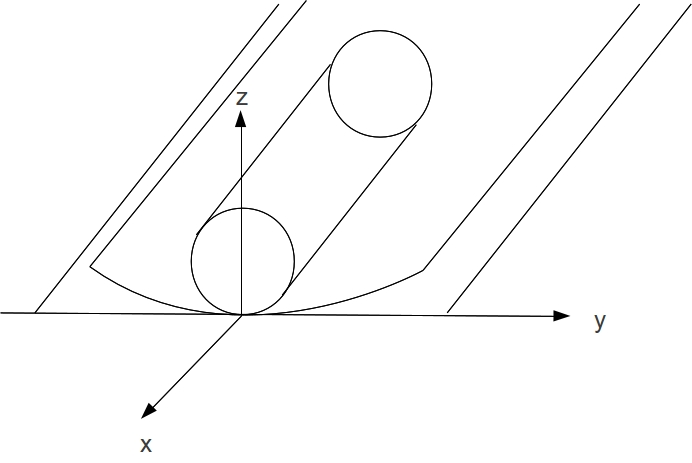
\includegraphics[scale = 0.3]{Bilder/Bsp7.jpg}
  \end{figure}
  \begin{align*}
   (u,v) \in ]-\pi, \pi[ \times \IR \mapsto x(u,v) = \vxyz{h \cdot v}{r \sin u}{r (1-\cos u)} \in \IR^3
  \end{align*}
  ist in die Ebene verbiegbar: Eine stetige Verbiegungsschar ist
  \begin{align*}
   \,^\alpha x(u,v) &= \vxyz{h v}{r \frac1\alpha \sin \alpha u}{r \frac1\alpha (1-\cos \alpha u)} \quad \alpha \in ]0,1] \\
   \,^0 x(u,v) &= \lim_{\alpha \to 0} \,^\alpha x(u,v) = \vxyz{hv}{ru}{0} \quad \text{[Ebenenstück], denn} \\
   \,^\alpha x_1(u,v) &= \vxyz{0}{r\cos \alpha u}{r\sin \alpha u} \\
   \,^\alpha x_2(u,v) &= \vxyz{h}{0}{0} \\
   \Rightarrow \big( \,^\alpha g_{\varrho \sigma}(u,v)\big) &= \begin{pmatrix}
                                                                  r^2 & 0 \\
                                                                  0 & h^2
                                                                 \end{pmatrix}
  \end{align*}
  Die \uline{Tangentialfläche}
  \[
   (s,v) \in I \times \IR \mapsto x(s,v) = c(s) + v T(s) \in \IR^3
  \]
  einer beliebigen wendepunktfreien Kurve \(s \mapsto c(s)\) ist in die Ebene verbiegbar. Es gilt
  \begin{align*}
   \big( \grs(s,v)\big) = \begin{pmatrix}
                           1 + v^2 \kappa^2(s) & 1 \\
                           1 & 1
                          \end{pmatrix}
  \end{align*}
  Die Torsion \(\tau\) der Kurve taucht nicht auf! Nach dem Fundamentalsatz der Kurventheorie kann eine von einem Parameter \(\alpha\) \uline{stetig} abhängende Kurvenschar \(s \mapsto \,^\alpha c(s)\) (\(\alpha \in [0,1]\)) durch Vorgabe von \(s \mapsto \,^\alpha \kappa(s) := \kappa(s)\) und \(s \mapsto \,^\alpha \tau(s) := \alpha \cdot \tau(s)\) konstruiert werden. Die zugehörigen Tangentenflächen bilden eine stetige Verbindungsschar zwischen einem Ebenenstück (\(=\) Tangentenfläche der ebenen Kurve \(\,^0 c\)) und der Ausgangsfläche (\(\alpha = 1\)).
 \end{enumerate}
\end{bsp}

\begin{bemerkung}
 Wir zeigen später, dass die
 \begin{itemize}
  \item \uline{allgemeinen Zylinder}, die 
  \item \uline{allgemeinen Kegel} und 
  \item \uline{Tangentenflächen von Kurven}
 \end{itemize}
 im wesentlichen die einzigen Flächen im \(\IR^3\) sind, die in die Ebene verbiegbar sind. \\
 Name: "`\uline{Torsen}"' \par
 Die Kugel ist \uline{nicht} isometrisch zur Ebene. Deswegen Ärger bei Atlanten (Atlassen).
\end{bemerkung}

\subsection{Hyperflächen im euklidischen $\IR^n$: Ableitungsgleichungen}
Im Folgenden sei \(\uline{p = n-1}\) \qquad 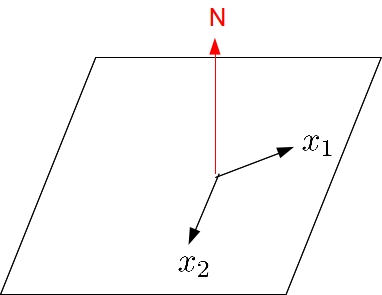
\includegraphics[scale=0.2]{Bilder/Bsp8.jpg}
Offensichtlich gilt

\begin{satz}\label{satz212}
 Ist \(u \in G \mapsto x(u) \in \IR^n\) Parameterdarstellung einer \(\C^1\)-Hyperfläche, so bilden die 
 \begin{itemize}
  \item tangentialen Vektorfelder
  \[
   x_1, \dots, x_{n-1}
  \]
  \item das Normalen(einheits)vektorfeld
  \[
   N := \frac{x_1 \times \dots \times x_{n-1}}{|x_1 \times \dots \times x_{n-1}|}
  \]
 \end{itemize}
 eine \uline{parameterabhängige}, positiv orientierte Begleitbasis\index{Hyperfläche!Begleitbasis} mit den Eigenschaften
 \begin{align*}
  \forall_\varrho \langle x_\varrho, N \rangle &= 0, \quad |N|^2 = 1 \\
  \det (x_1, \dots, x_{n-1}, N) &= \langle x_1 \times \dots \times x_{n-1}, N \rangle = |x_1 \times \dots \times x_{n-1} | = \sqrt{g} = a_{n-1} (x_1, \dots, x_{n-1})
 \end{align*}
 Das Vektorfeld \(N \colon G \to S^{n-1} \subset \IR^n\) ist dabei invariant gegenüber (zulässiger) Parametertransformationen und heißt auch \uline{sphärisches Bild}\index{sphärisches Bild} oder \uline{Gaußabbildung}\index{Gaußabbildung} der Hyperfläche.
\end{satz}

\begin{bemerkung}
 In jedem Punkt \(x(u)\) ist die orthogonale Zerlegung
 \[
  \IR^n = T_u x \stackrel{\perp}{\oplus} \hl N \hr
 \]
 parameterunabhängig.
\end{bemerkung}

\begin{satz}\label{satz213}
 Für die Begleitbasis \((x_1, \dots, x_{n-1}, N)\) einer parametrisierten \(\C^2\)-Hyperfläche gelten (parameter\-\uline{abhängige}) Ableitungsgleichungen der Form 
 \begin{align*}
 &\boxed{\underset{\varrho, \sigma}{\forall}\, x_{\varrho \sigma} = \sum \gamma_{\varrho \;\, \sigma}^{\;\,\mu}\, x_\mu + b_{\varrho \sigma} N} \\
 &\text{[Gaußsche Ableitungsgleichungen]\index{Gaußsche Ableitungsgleichungen]}} \\
 &\boxed{N_\sigma := \partial_\sigma N = - \sum b^\mu_{\;\, \sigma}\, x_\mu [ + 0 \cdot N]} \\
 &\text{[Weingartenschen Ableitungsgleichungen]\index{Weingartenschen Ableitungsgleichungen}}
 \end{align*}
\end{satz}

\begin{beweis}[von Satz \ref{satz213}]
 Klar wegen 
 \[
  |N|^2 = 1 \Rightarrow \langle N_\sigma, N \rangle = 0
 \]
\end{beweis}

\subsubsection*{Berechnung der Koeffizienten}
\begin{enumerate}
 \item[a)] Mit den \uline{Christoffelsymbolen\index{Christoffelsymbole} 1. Art}
 \[
  \gamma_{\varrho \nu \sigma} := \langle x_{\varrho \sigma}, x_\nu \rangle = \sum_\mu \gamma_{\varrho \;\, \sigma}^{\;\,\mu} \, g_{\mu \nu}
 \]
 erhält man die \uline{Christoffelsymbole 2. Art} durch
 \[
  \christ \varrho \mu \sigma = \sum_\nu g^{\mu\nu} \, \gamma_{\varrho \nu \sigma}
 \]
 wenn \((g^{\mu\nu})\) die zur \((g_{\varrho \sigma})\) inverse Matrix (mit \(\sum_\nu g^{\mu\nu} \, \grund \nu\sigma = \delta^\mu_{\;\, \nu}\)) berechnet.
 \item[b)] Es gilt
 \begin{align*}
  b_{\varrho\sigma} &= \langle x_{\varrho\sigma}, N \rangle = -\langle x_{\varrho}, N_\sigma \rangle = + \sum_\mu b^\mu_{\;\,\sigma} \, g_{\mu \varrho} \\
  \Rightarrow b^\mu_{\;\,\sigma} &= \sum_{\varrho} g^{\mu\varrho} \, b_{\varrho\sigma}
 \end{align*}
\end{enumerate}

\begin{bemerkung}\(\)
\begin{enumerate}
 \item Mit den Matrizen \((g_{\varrho\sigma})\) und ihrer Inversen \((g^{\varrho \sigma})\) lassen sich im Tensorkalkül Indizes "`herauf- und herunterziehen"'.
 \item \((\gamma_{\varrho\nu\sigma}),\, (\gamma_{\varrho \;\, \sigma}^{\;\,\mu}),\, (v_{\varrho \sigma})\) sind in dem Indexpaar \((\varrho, \sigma)\) \uline{symmetrisch}.
 \begin{align*}
 (b^\mu_{\;\,\sigma}) = (g^{\mu\nu}) \cdot (b_{\varrho \sigma})
 \end{align*}
 braucht \uline{nicht} symmetrisch sein, obwohl Produkt symmetrischer Matrizen!
 \item Bei \(n = 3\) denke man an \(N = \frac1{\sqrt{g}} x_1 \times x_2\)
 \begin{align*}
 (g^{\varrho \sigma}) &= \frac1g \begin{pmatrix}
                                 g_{22} & -g_{12}\\
                                 -g_{21} & g_{11}
                                \end{pmatrix} \\
 (b^\mu_{\;\,\sigma}) &= \begin{pmatrix}
                        b^1_{\;\,1} & b^1_{\;\,2} \\
                        b^2_{\;\,1} & b^2_{\;\,2}
                       \end{pmatrix}         
 \end{align*}
\end{enumerate}

\end{bemerkung}

\subsubsection*{Fragen}
\begin{enumerate}
 \item Welche geometrische und algebraische Bedeutung haben die Koeffizienten \(\gamma_{\varrho \;\, \sigma}^{\;\,\mu}, \, b_{\varrho\sigma},\, b^\mu_{\;\,\sigma}\)?
 \item Wie ändern sie sich bei Parametertransformationen? (z.T. kompliziert, Berechnung soll vermieden werden)
 \item Wie kann man die Ableitungsgleichungen parameterunabhängig formulieren?
\end{enumerate}

\subsubsection*{Idee (zu 3.)}
Statt die parameterabhängigen Vektorfelder \(x_1, \dots, x_{n-1}, N\) in Richtung von Parameterlinien (nach \(u^\sigma\)) zu differenzieren, Ableiten eines \uline{beliebigen} (tangentialen oder normalen) Vektorfeldes \(u \mapsto Z(u)\) in Richtung eines \uline{beliebigen} Vektors \(Y \in T_u x\). Diese \uline{Richtungsableitung}\index{Richtungsableitung}
\begin{align*}
 \boxed{\dd_Y Z = \sum (\partial_\sigma Z) Y^\sigma}
\end{align*}
(mit \(Y = \sum Y^\sigma x_\sigma\)) [vergleiche im \(\IR^n\): \(d_Y f = \langle \grad f, Y \rangle = \sum \partial_\varrho f \cdot Y^\varrho\)]\par
ist \uline{parameterunabhängig}, denn aus \(x = \widetilde x \circ \Phi, \, Z = \widetilde Z \circ \Phi, \, Y = \widetilde Y \circ \Phi\) folgt	
\begin{align*}
 &\dd_Y Z(u) = \sum_\sigma \partial_\sigma \left( \widetilde Z \big( \Phi(u)\big)\right) Y^\sigma(u) = \sum_{\mu,\sigma} \left( \partial_\mu \widetilde Z\right) \big(\Phi(u)\big) \underbrace{\frac{\partial \widetilde u^\mu}{\partial u^\sigma} Y^\sigma(u)}_{\widetilde Y^\mu \big(\Phi(u)\big)} = \uline{\dd_{\widetilde Y} \widetilde Z} \big(\Phi(u)\big) \\
 &\left(\text{weil } x_\varrho = \sum \widetilde u_\varrho^\sigma \,\widetilde x_\sigma \Leftrightarrow \widetilde Y^\sigma = \sum \widetilde u_\varrho^\sigma \, Y^\varrho\right)
\end{align*}

\subsubsection{Eigenschaften des linearen Differentialoperators}
\[
 d \colon (Z,Y) \mapsto \dd_Y Z
\]
\begin{enumerate}
 \item[1a)] Additivität in \(Z\):
 \[
  \dd_Y (Z_1 + Z_2) = \dd_Y Z_1 + \dd_Y Z_2
 \]
 \item[1b)] Derivativität in \(Z\):
 \[
  \dd_Y(f \cdot Z) = (\dd_Y f)Z + f \dd_Y Z
 \]
 \item[2)] Linearität in \(Y\):
 \[
  \dd_{f_1 Y_1, f_2 Y_2} Z = f_1 \dd_{Y_1} Z + f_2 \dd_{Y_2} Z
 \]
\end{enumerate}
Da auch die Zerlegung von \(u \mapsto \dd_Y Z(u)\) in Tangential- und Normalanteil parameterunabhängig ist, erhält man folgende invariante Darstellung: \par
Für \(Z = X\) selbst tangential gilt
\begin{align*}
 \dd_Y X &= \sum \partial_{\sigma} \left( \sum X^{\cancelto{\mu}{\varrho}} x_{\cancelto{\mu}{\varrho}}\right)Y^\sigma = \sum \left( \partial_\sigma X^\varrho \right) Y^\sigma x_\varrho + \sum X^\varrho x_{\varrho \sigma} X^\sigma \\
 &=\underbrace{\sum \left[ \left( \partial_\sigma X^\mu + X^\varrho \christ \varrho \mu \sigma \right) Y^\sigma \right] x_\mu}_{\dd_Y X |_\perp} + \underbrace{\left[ \sum b_{\varrho \sigma} X^\varrho Y^\sigma \right]}_{\langle \dd_Y X, N\rangle = \langle- X, \dd_Y N \rangle (\text{(Bilinearform)})} N \\
 &=: \nabla_Y X + \Rom 2 (X,Y) N
\end{align*}
und für \(Z = N\):
\begin{align*}
 \dd_Y N = \sum \left( \partial_\sigma N\right) Y^\sigma = - \sum \wein \mu \sigma Y^\sigma x_\mu = -A(Y) \quad \text{(lineare Abbildung)}
\end{align*}

\uline{Ergebnis}:

\begin{satz}\label{satz214}
 Auf einer \(\C^2\)-Hyperfläche in einer Parametrisierung \(u \mapsto x(u) \) erfüllen tangentiale \(\C^1\)-Vektorfelder \(u \mapsto X(u)\) un das Normalenvektorfels \(u \mapsto N(u)\) die (parameterunabhängigen) \uline{Ableitungsgleichun}\-\uline{gen}
\begin{align*}
 \dd_Y X &= \nabla_Y X + \Rom 2 (X,Y) N & \text{(Gaußsche Ableitungsgleichung)} \\
 \dd_Y N &= -A (Y) & \text{(Weingartensche Ableitungsgleichung)}
\end{align*}
in Richtung tangentialer Vektorfelder \(u \mapsto Y(u)\). \par
Dabei gilt:
\begin{enumerate}
 \item[a)] Durch \((X,Y) \mapsto \nabla_Y X = \dd_Y X |_T\) wird ein linearer Differentialoperator definiert, der je zwei tangentialen Vektorfeldern \(X,Y\) wieder ein tangentiales Vektorfeld \(\nabla_Y X\) zuordnet, genannt \uline{kovariante Ableitung}\index{kovariante Ableitung} von \(X\) in Richtung \(Y\). \\
 (Andere Bezeichnung: Durch \(\nabla\) wird ein \uline{linearer Zusammenhang}\index{linearer Zusammenhang} (linear connection) definiert)
 \item[b)] Durch \((X,Y) \mapsto \Rom 2(X,Y) = \langle \dd_Y X, N\rangle = -\langle X, \dd_Y N \rangle = -\Rom 1 (X, \dd_YN)\) wird ein Feld symmetrischer \uline{Bilinearformen} 
 \[
  \Rom 2_u \colon T_u x \times T_u x \to \IR, \, (X,Y) \mapsto \Rom 2_u (X,Y)
 \]
 definiert, genannt \uline{2. Grundform}\index{2. Grundform} (2. Fundamentalform) der Hyperfläche
 \item[c)] Durch \(Y \mapsto A(Y) := -\dd_Y N\) wird ein Feld \uline{linearer Abbildungen} \(A_u \colon T_u x \to T_u x\) definiert, genannt \uline{Weingarten-Endomorphismus}\index{Weingarten-Endomorphismus} (shape operator) der Hyperfläche.
\end{enumerate}

\end{satz}

\begin{folgerung}[Interpretation von \(\christ \varrho \mu \sigma\), \(b_{\varrho \sigma}\), \(\wein \mu \sigma\)]
 Bezüglich einer festen Parametrisierung \(u \mapsto x(u)\) einer \(\C^2\)-Hyperfläche hat man die Basisdarstellung (setze \(X = X_\varrho, Y = X_\sigma\))
 \begin{align*}
  \nabla_\sigma X_\varrho &:= \nabla_{x_\sigma} x_\varrho = \sum \christ \varrho \mu \sigma x_\mu \\
  \Rom 2 (x_\varrho, x_\sigma) &= b_{\varrho \sigma} \\
  A(x_\sigma) &= + \sum \wein \mu \sigma x_\mu
 \end{align*}
Die Christoffelsymbole \(\christ \varrho \mu \sigma\) sind also die \uline{Darstellungskoeffizienten} der kovarianten Ableitung \(\nabla\) (auch als \uline{Zusammenhangskoeffizienten} bezeichnet), \\
die symmetrische Matrix \((b_{\varrho \sigma})\) ist die \uline{Darstellungsmatrix} der 2. Grundform \(\Rom 2\) und \\
die (im Allgemeinen nicht symmetrische) Matrix \((\wein \mu \sigma )\) die \uline{Darstellungsmatrix} des Weingarten-Endomorphismus \(A\), jeweils bezüglich der Basisfelder \(u \mapsto \big(x_1, \dots, x_{n-1}\big) (u)\) \par
Umgekehrt gilt (bezüglich jeder Parametrisierung):
\begin{align*}
 \nabla_Y X &= \sum \left[ \partial_\sigma X^\mu + X^\varrho \christ \varrho \mu \sigma Y^\sigma \right] x_\mu \\
 \Rom 2 (X,Y) &= \sum b_{\varrho \sigma} X^\varrho Y^\sigma \\
 A(Y) &= \sum \wein \mu \sigma Y^\sigma x_\mu
\end{align*}
Früher übliche Bezeichnung für \(p = 2, n = 3\)
\[
 (b_{\varrho \sigma}) = \begin{pmatrix}
                        L & M \\
                        M & N
                       \end{pmatrix} = 
                       \begin{pmatrix}
                        e & f \\
                        f & g
                       \end{pmatrix}
\]
\end{folgerung}

(Für Profis: \(\nabla\) ist der von der Metrik \(\Rom 1\) induzierte Levi-Civita-Zusammenhang.)

\subsubsection{Grundlegende Eigenschaften von \(\nabla, \, \Rom 2, \, A\)}
\begin{enumerate}
 \item[(1)] Die kovariante Ableitung \(\nabla\) (bezüglich ihrer Koeffizienten \(\christ \varrho \mu \sigma\)) ist eine \uline{innergeometrische Größe}
\end{enumerate}

\begin{satz}\label{satz215}
 Die Christoffelsymbole 1. und 2. Art einer \(\C^2\)-(Hyper)Fläche lassen sich allein aus den Komponenten \(g_{\varrho \sigma}\) der 1. Grundform bestimmen. Und zwar gilt
 \begin{align*}
  \gamma_{\varrho \nu \sigma} &= \frac12 \left( \partial_\varrho g_{\nu \sigma} - \partial_\nu g_{\varrho \sigma} + \partial_\sigma g_{\varrho \nu}\right) \\
  \christ \varrho \mu \sigma &= \sum g^{\mu \nu} \gamma_{\varrho \nu \sigma}
 \end{align*}
\end{satz}

\begin{beweis}[von Satz \ref{satz215}]
 Aus 
 \begin{align*}
  \partial_\varrho g_{\nu \sigma} &= \partial_\varrho \langle x_\nu, x_\sigma \rangle = \langle x_{\nu \varrho}, x_\sigma \rangle + \langle x_\nu, x_{\sigma \varrho} \rangle &= \gamma_{\nu\sigma\varrho} + \gamma_{\sigma \nu \varrho} \\
  \partial_\nu g_{\varrho \nu} &= \dots &= \gamma_{\varrho \sigma \nu} + \gamma_{\sigma \varrho \nu} \\
  \partial_\sigma g_{\varrho \nu} &= \dots &= \gamma_{\nu \varrho \sigma} + \gamma_{\varrho \nu \sigma}
 \end{align*}
 und der Symmetrie \(\gamma_{\varrho \nu \sigma} = \gamma_{\sigma \nu \varrho}\) die Behauptung.
\end{beweis}

\begin{enumerate}
 \item[(2)] Die Weingarten-Matrizen \((\wein \mu \sigma )\) bezüglich verschiedener Parametrisierungen sind (als Darstellungsmatrizen desselben Endomorphismus \(A\)) \uline{ähnlich} zueinander. \\
 (Parameterunabhängige) \uline{Invarianten} sind also ihre elementarsymmetrischen Funktionen (\(=\) Koeffizienten des charakteristischen Polynoms), insbesondere Spur und Determinante.
\end{enumerate}

\begin{definition}
 Bei einer \(\C^2\)-Hyperfläche im \(\IR^n\) heißt 
 \[
  H:= \frac{1}{n-1} \tr A = \frac{1}{n-1} \sum \wein \varrho \varrho
 \]
 die \uline{mittlere Krümmung}\index{mittlere Krümmung} und
 \[
  \kappa := \det A = \det (\wein \mu \sigma)
 \]
 die \uline{Gaußsche Krümmung}\index{Gaußsche Krümmung}
\end{definition}

\begin{bemerkung}
 Aus \((\wein \mu \sigma ) = (g^{\stackrel{\alpha}{\varrho}\stackrel{\beta}{\sigma}}) \cdot (b_{\varrho \sigma})\) folgt 
 \[
  \kappa = \frac{b}{g} = \frac{\det (b_{\varrho \sigma})}{\det (g_{\varrho \sigma})}
 \]
\end{bemerkung}

\begin{enumerate}
 \item[(3)] Der Weingarten-Endomorphismus \(A\) ist \uline{selbstadjungiert}. Für tangentiale Vektorfelder \(X,Y\) gilt \(\langle X, Y\rangle = 0\), also 
 \begin{align*}
  \dd_Y \left[ \langle X,N \rangle \right] &= \langle \dd_Y X, N \rangle + \langle X, \dd_Y N \rangle = \Rom 2 (X,Y) - \langle X;A(Y) \rangle \\
  &=\Rom 2 (X,Y) - \Rom 1\big(Y, A(Y)\big) = 0 \\
  (\text{in Koordinaten: } &= b_{\varrho \sigma} - \sum g_{\varrho \mu} \wein \mu \sigma )
  \end{align*}
  Die Symmetrie von \(\Rom 2\) liefert
\end{enumerate}

\begin{satz}\label{satz216}
 Die Weingartenabbildung \(A_u \colon T_u x \to T_u x\) ist in jedem Punkt \(x(u)\) einer Hyperfläche \uline{selbstadjungiert} bezüglich des Skalarprodukts \(\Rom 1_u\) auf \(T_u x\), d.h. es gilt überall
 \[
  \Rom 1 \big(X, A(Y)\big) = \Rom 1 \big(A(X), Y\big)
 \]
 Sie besitzt demnach nur \uline{reelle Eigenwerte} und eine \uline{Orthonormalbasis aus Eigenvektoren}.
\end{satz}

\begin{bemerkung}
 Obwohl \(A\) selbstadjungiert ist, sind die Darstellungsmatritzen \((\wein \mu \sigma)\) in \(A\) nicht \uline{symmetrisch}.
\end{bemerkung}

\subsubsection{Bezeichnungen}
Eigenwert von \(A_u\):
\[
 \kappa_1(u), \dots, \kappa_{n-1}(u) \quad \text{\uline{Hauptkrümmungen}}
\]
Orthonormierte Eigenvektoren dazu:
\[
 Y_1(u), \dots, Y_{n-1}(u) \quad \text{\uline{Hauptkrümmungsrichtungen}}
\]

\subsubsection{Zusammenfassung Krümmungsinvarianten aus den Weingartenabbildungen \(Y \mapsto A(Y) = -\dd_Y N\)}
\begin{align*}
 &H = \frac{1}{n-1} \tr A & \text{Mittlere Krümmung} \\
 &\kappa = \det A & \text{Gaußsche Krümmung} \\
 &\kappa_1, \dots, \kappa_{n-1} & \text{Hauptkümmungen = Eigenwerte von }A \\
 &Y_1, \dots, Y_{n-1} & \text{Hauptkrümmung = Eigenvektoren von }A \text{(Orthonormalbasis!)}
\end{align*}

\begin{folgerung}
 Wegen \(A(Y_\varrho) = \kappa_\varrho Y_\varrho (\varrho = 1, \dots, n-1)\) gilt
 \begin{align*}
  &H = \frac{1}{n-1} (\kappa_1 + \dots + \kappa_{n-1} & \text{(deswegen \uline{mittlere} Krümmung)} \\
  & \kappa = \kappa_1 \cdot \dots \cdot \kappa_{n-1}
 \end{align*}
Zur geometrischen Bedeutung: siehe Kapitel 2.3
\end{folgerung}

\subsubsection{Vorgriff ($n=3$)}
Flächen mit \(H \equiv 0\) heißen \uline{Minimalflächen} \\
Flächen mit \(\kappa \equiv 0\) heißen \uline{Torsen} (\(=\) ``flache Flächen'') \\
Formelsammlung: siehe Homepage J. König.
\subsubsection{Ergänzung}
Oft sind tangentiale Vektorfelder nur längs einer Flächenkurve \(t \mapsto c(t) = x\big(u(t)\big)\) in der Form 
\[
 t \mapsto X(t) = \sum X^\varrho(t)x_{\varrho}\big(u(t)\big)
\]
gegeben.
\begin{bsp}
  \mat{X(t) := \dot c(t) = \sum \dot u^\varrho(t)x_\varrho \big(u(t)\big)}
  \uline{kovariante Ableitung}:
  \begin{align*}
   \frac{\nabla X}{\dd t} &:= \left.\frac{\dd X}{\dd t} \right|_T = \sum \left[\dot X^{\cancelto{\mu}{\varrho}} x_{\cancelto{\mu}\varrho} \;\,(u) + X^\varrho x_{\varrho \sigma} (u)|_\perp \cdot \dot u^\sigma\right] \\
   &= \uline{\sum \left( \dot X^\mu + X^\varrho \christ \varrho \mu \sigma (u) \dot u^\sigma \right) x_\mu(u)}
  \end{align*}
\end{bsp}

\section{Zur inneren Geometrie der Flächen im $\IR^3$}
Im Folgenden sei \(p = 2, n = 3\); das meiste gilt für beliebige \(p\). \par
In der euklidischen Ebene sind wohldefinierte:
\begin{itemize}
 \item die \uline{Parallelverschiebung}\index{Parallelverschiebung} eines Vektors \(X_0\) längs einer Kurve \(t \mapsto c(t)\). Sie liefern ein \uline{Parallelfeld}\index{Parallelfeld} \(t \mapsto X(t)\) mit \(\frac{\dd X}{\dd t} = 0\), d.h. \(X = X_0 = \const.\)
 \item \uline{gerade Linien}, etwa mit der Kennzeichnung \(\frac{\dd T}{\dd t} \equiv 0\), d.h. \(T = \const.\)
\end{itemize}
Übertragung der Begriffe auf ``krumme'' Flächen durch Rückprojektion der Ableitungsvektoren \(\frac{\dd X}{\dd t}\) bzw. \(\frac{\dd T}{\dd t}\) in die Tangentialebene, d.h. Benutzung der (innergeometrischen) kovarianten Ableitung \(\frac{\nabla X}{\dd t}\) bzw. \(\frac{\nabla T}{\dd t}\). \\
(Vektorfelder sind nur so parallel bzw. Kurven nur so gerade, wie die Fläche es zulässt.

\subsection{Geodätische Parallelverschiebung}
\Rechts
\begin{definition}
 Ein tangentiales \(\C^1\)-Vektorfeld \(t \mapsto X(t) = \sum X^\varrho (t) x_\varrho \big(u(t)\big)\) längs einer \(\C^1\)-Flächenkurve \(t \mapsto c(t) = x\big(u(t)\big)\) heißt \uline{geodätisch parallel}\index{geodätische Parallelität}, wenn gilt
 \begin{align*}
  &\frac{\nabla X}{\dd t} = \left.\frac{\dd X}{\dd t}\right|_T \equiv 0, \text{ also} \\
  &\dot X^\mu + \sum X^\varrho \christ \varrho \mu \sigma (u) \dot u^\sigma = 0 \quad (\mu = 1,2) \tag{\(\ast\)}
 \end{align*}
(d.h. der innergeometrisch nur sichtbare Anteil der Ableitung verschwindet) \par
\((\ast)\) ist ein \uline{lineares} Differentialgleichungssystem 1. Ordnung für die Komponentenfunktionen \(t \mapsto X^\mu (t)\, (\mu = 1,2)\), das unter Anfangsbedingungen \(X^\mu(t_0) = X_0^\mu\, (\mu = 1,2)\) eindeutig gelöst werden kann.5
\end{definition}

\begin{folgerung}
 Ein Tangentialvektor auf einer \(\C^2\)-Fläche lässt sich längs jeder \(\C^1\)-Flächenkurve eindeutig geodätisch parallelverschieben. Bei Parallelverschiebung bleiben metrische Größen erhalten:
\end{folgerung}

\begin{satz}\label{satz221}
 Sind \(t \mapsto X(t) = \sum X^\varrho (t) x_\varrho\big(u(t)\big), \, Y(t) = \sum X^\sigma(t) x_\sigma \big(u(t)\big)\) geodätisch parallele \(\C^1\)-Vektorfelder längs derselben \(\C^1\)-Flächenkurve \(t \mapsto c(t) = x\big(u(t)\big)\), so gilt
 \begin{align*}
  t \mapsto \Rom 1_{u(t)}\big(X(t), Y(t)\big) = \sum g_{\varrho \sigma} \big(u(t)\big) X^\varrho(t) Y^\sigma(t) = \const.
 \end{align*}
d.h. Längen, Winkel, Flächeninhalt bleiben erhalten.
\end{satz}
Der Satz kann ``innergeometrisch'' bewiesen werden. \\
kürzer: ``außergeometrisch''

\begin{beweis}[von Satz \ref{satz221}]
 \begin{align*}
  \frac{\dd}{\dd t} \left( \Rom 1_{u(t)} \big( X(t), Y(t) \big)\right) &= \frac{\dd}{\dd t} \langle X(t), Y(t)\rangle = \left\langle \frac{\dd X}{\dd t}(t), Y(t) \right\rangle + \left\langle X(t), \frac{\dd Y}{\dd t}(t)\right\rangle \\
  &= \left\langle \underbrace{\frac{\nabla X}{\dd t} (t)}_{=0}, Y(t) \right\rangle + \left\langle X(t), \underbrace{\frac{\nabla Y}{\dd t}(t)}_{=0} \right\rangle =0
 \end{align*}

\end{beweis}

\begin{bsp}[für geodätische Parallelfelder (ohne Rechnung!)]
 Benutzte Eigenschaften:
 \begin{enumerate}
  \item In der \uline{Ebene} gilt ``parallel'' = ``geodätisch parallel''
  \item \uline{Berühren} sich zwei Flächen längs einer Flächenkurve, so ist der geodätische Parallelismus bezüglich dieser Kurven für beide Flächen derselbe (denn es wird in die gleiche Tangentialebene projeziert)
 \end{enumerate}
\uline{Kreiszylinder} 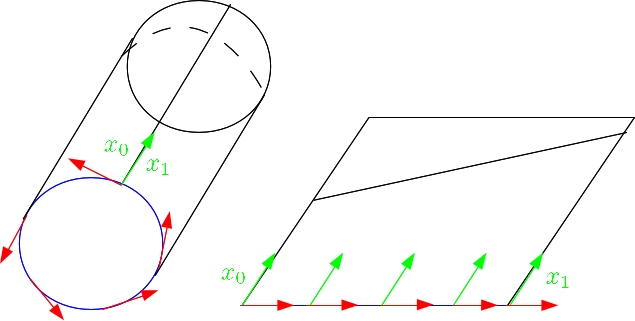
\includegraphics[scale=0.2]{Bilder/Bsp9} \par
\uline{Kreiskegel} 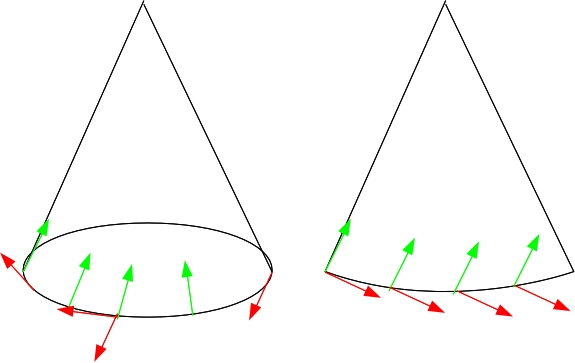
\includegraphics[scale=0.2]{Bilder/Bsp10} \par
\uline{Großkreis} 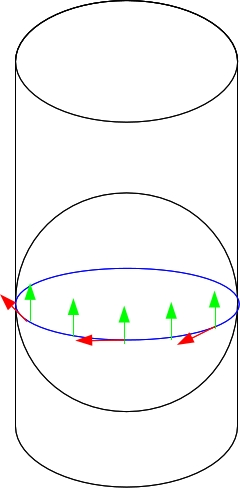
\includegraphics[scale=0.2]{Bilder/Bsp11} 
grüne Pfeile: Parallelfeld längs Großkreis \\
roter Pfeil: Tangentenvektoren bilden Parallelfeld (berühren Zylinder) \par
\uline{Kleinkreis} 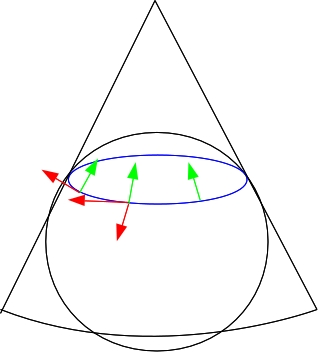
\includegraphics[scale=0.2]{Bilder/Bsp12}
grüner Pfeil: Parallelfeld längs Kleinkreis \\
roter Pfeil: Tangentenvektoren bilden \uline{kein} Parallelfeld \par
Geodätische Parallelverschiebung ist im Allgemeinen nicht wegunabhängig. 
\begin{figure}[ht]
 \centering
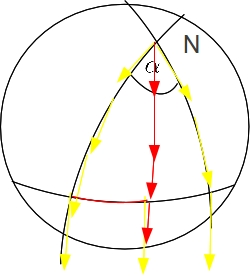
\includegraphics[scale=0.3]{Bilder/Bsp13}
\end{figure}
\end{bsp}

\subsection{Geodätische Linien}
\begin{definition}
 Eine \uline{Geodätische}\index{Geodätische} (Autoparallele, ``Geodäte'') auf einer \(\C^2\)-Fläche ist eine \(\C^2\)-Flächenkurve mit geodätisch parallelem Tangenteneinheitsfeld, d.h. mit
 \[
  \boxed{\frac{\nabla T}{\dd t} \equiv 0}
 \]
\end{definition}
\begin{bsp} \(\)
 \begin{enumerate}
  \item Schraubenlinien auf Kreiszylindern (\(\widehat{=}\) Geraden in der Abwickelebene)
  \item Großkreise auf Kugeln, aber nicht andere Kreise.
 \end{enumerate}
\end{bsp}
Aus \(\dot c = w T\) (mit \(w = |\dot c|\)) folgt 
\begin{align*}
 \frac{\nabla \dot c}{\dd t} = w \cdot \frac{\nabla T}{\dd t} + \dot w T
\end{align*}
und wegen 
\[ 
\Rom 1 \left(T, \frac{\nabla T}{\dd t}\right) = \left\langle T, \frac{\dd T}{\dd t} \right\rangle = 0
\]
gilt
 \begin{align*}
  \frac{\nabla \dot c}{\dd t} \equiv 0 &\Leftrightarrow \frac{\nabla T}{\dd t} = 0 \land \dot w = 0 \\
  &\Leftrightarrow c \text{ ist Geodätische, proportional zur Bogenlänge parametrisiert}
 \end{align*}

Für Flächenkurven in BLP \(s \mapsto c(s)\) gilt natürlich:
\[
 c \text{ Geodätische } \Leftrightarrow \frac{\nabla c'}{\dd s} \equiv 0
\]
\Links
\begin{folgerung}
 Geodätische in \(\C^2\)-BLP \(s \mapsto c(s)\), d.h. mit
 \[
  |c'|^2 = \sum g_{\varrho \sigma}(u) u'^\varrho u'^\sigma \equiv 1
 \]
 sind (in der Parameterebene) gekennzeichnet durch
 \begin{align*}
  u''^\mu + \sum_{\varrho, \sigma} \christ \varrho \mu \sigma (u) u'^\varrho u'^\sigma \equiv 0  \quad (\mu = 1,2) \tag{\(\ast\)}
 \end{align*}
\big(Differentialgleichungssystem für \(s \mapsto u^1(s), u^2(s)\)\big)
\end{folgerung}

\begin{beweis}[der Folgerung]
 \begin{align*}
  \frac{\nabla c'}{\dd s} &= \frac{\nabla}{\dd s} \left(\sum u'^\varrho x_\varrho(u) \right) = \sum u''^{\cancelto{\mu}{\varrho}} x_{\cancelto{\mu}{\varrho}} \;(u) + \sum u'^\varrho \nabla_{\sigma} x_\varrho (u) u'^\sigma \\
  &= \sum \left(u''^\mu + \christ \varrho \mu \sigma (u) u'^\varrho u'^\sigma \right) x_\mu (u) \equiv 0 \Leftrightarrow (\ast)
 \end{align*}
\end{beweis}

Zur Existenz von Geodätischen:

\begin{satz}\label{satz222}
 Auf einer \(\C^3\)-Fläche verläuft durch \uline{jeden} Flächenpunkt in \uline{jede} Tangentialrichtung \uline{genau eine} Geodätische.
\end{satz}

\begin{beweis}[von Satz \ref{satz222}]
 \((\ast)\) bildet ein im Allgemeinen \uline{nichtlineares} autonomes Differentialgleichungssystem 2. Ordnung für die Funktionen \(s \mapsto u^1(s), u^2(s)\) (transformierbar in ein System 1. Ordnung). Es besitzt etwa für \(\C^3\)-Flächen (mit \(\C^1\)-Christoffelsymbolen \(\Rightarrow\) lokale Lipschitzbeschränktheit) zu vorgegebenen Anfangsbedingungen \(u^\mu(0) = u_0^\mu, u'^\mu(0) = X_0^\mu \,(\mu = 1,2)\) genau eine auf einem maximalen Intervall um \(s = 0\) definierte Lösung \(s \in I \mapsto u(s) = \big(u^1(s),u^2(s)\big) \in G \subset \IR^2\). Also existiert genau eine Geodätische \(s \in I \mapsto c(s) = x\big( U(s)\big) \in M \subset \IR^3\) mit \(c(0) = x(u_o) = x_0\) und \(c'(0) = \sum X_0^\mu x_\mu(u_0) = X_0 \in T_{u_0}x\) (wenn \(|X_0| = 1\))
\end{beweis}

\begin{bemerkung}
 Die maximal fortgesetzte Lösung  \(s \in I \mapsto u(s) \in G \subset \IR^2\) braucht nur auf einem endlichen Intervall \(I = ]s_{-}; s_{+}[\) definiert zu sein. Die zugehörige Geodätische besitzt dann \uline{endliche Länge}. Flächen, auf denen jede Geodätische \(\infty\)-lang ist (\(I = \IR\)) heißen \uline{geodätisch vollständig}\index{geodätische Vollständigkeit}.
\end{bemerkung}

Geodätische sind nach Definition ``möglichst gerade''. Sind sie auch ``möglichst kurz''?

\begin{satz}\label{satz223}
 Auf einer \(\C^2\)-Fläche ist eine kürzeste Verbindungskurve zwischen zwei festen Flächenpunkten notwendig eine Geodätische.
 \[
  \text{``möglichst kurz'' } \Rightarrow \text{ ``möglichst gerade''}
 \]
\end{satz}

\begin{beweis}[von Satz \ref{satz223}]
 Gegeben: \(\C^2\)-Flächenkurve \(st \mapsto c(t) = x\big(u(t)\big)\) mit \(\begin{cases}
                                                                            c(a) = x(u_a) = x_a \\
                                                                            c(b) = x(u_b) = x_b
                                                                           \end{cases}\). \par
 Wir konstruieren \(\C^2\)-Vergleichsflächenkurven \(t \mapsto \,^\varepsilon c(t) \, \big(\varepsilon \in U(0)\big)\) mit
 \[
  \forall_\varepsilon \,^\varepsilon c(a) = x_a, \, \,^\varepsilon c(b) = x_b, \, \,^\varepsilon c |_{\varepsilon = 0} = c
 \]
 und untersuchen ihre Längen \(L_a^b (\,^\varepsilon c)\). \par
 Ansatz: \(\,^\varepsilon c(t) = x\big( \,^\varepsilon u(t)\big) = x\big( u(t) + \varepsilon v(t)\big)\) mit einer \(\C^2\)-Abbildung \(t \in [a,b] \mapsto v(t) \in \IR^2\), wobei \(v(a) = v(b) = 0\) (diese sind regulär für genügend kleine \(\varepsilon\), d.h. \(|\,^\varepsilon \dot c(t) | > 0\)). \par
 Die Kurven definieren ein \uline{\(\C^1\)-Variationsvektorfeld}
 \[
  t \in [a,b] \mapsto V(t):= \frac{\partial}{\partial \varepsilon} \big(\,^\varepsilon \left.(c(t)\big)\right|_{\varepsilon = 0} = \sum v^\varrho(t) x_\varrho \big(u(t)\big) \in T_{u(t)}x
 \]
 mit \(V(a) = V(b) = 0\). \par
 Falls \(c\) kürzeste Verbindung zwischen \(x_a\) und \(x_b\), muss gelten
 \[
  \boxed{\frac{\dd}{\dd\varepsilon} \left.L_a^b (\,^\varepsilon c)\right|_{\varepsilon = 0} = 0}
 \]
 \big(und zwar für alle Abbildungen \(t \mapsto v(t)\)\big)
 \uline{Berechnung}:
 \begin{align*}
  \frac{\dd}{\dd \varepsilon} \left. L_a^b (\,^\varepsilon c) \right|_{\varepsilon = 0} &= \frac{\dd}{\dd \varepsilon} \left[ \int_a^b |\,^\varepsilon \dot c(t)| \dd t\right]_{\varepsilon = 0}\\
  &= \int_a^b \frac{\partial}{\partial \varepsilon} \left.\underbrace{|\,^\varepsilon \dot c(t)|}_{> 0} \dd t \right|_{\varepsilon = 0} = \int_a^b \frac1{|\,^\varepsilon c(t)|} \langle \,^\varepsilon c(t), \left.\underbrace{\partial_\varepsilon \dot c(t)}_{\partial_\varepsilon \partial_t \,^\varepsilon c(t)} \rangle \dd t \right|_{\varepsilon = 0} \\
  &= \int_a^b \frac{1}{|\dot c(t)|} \left\langle \dot c(t), \dot V(t) \right\rangle \dd t \\
  &= \int_a^b \left\langle T(t), \dot V(t) \right\rangle \dd t = \int_a^b \frac{\dd}{\dd t} \left\langle T(t) V(t) \right\rangle \dd t - \int_a^b \left\langle \dot T(t), V(t) \right\rangle \dd t \\
  &= \left. \left\langle T(t), V(t) \right\rangle \right|_a^b - \int_a^b \left\langle \frac{\nabla T}{\dd t}(t), V(t) \right\rangle \dd t \\
  &= -\int_a^b \Rom 1_{u(t)} \left( \frac{\nabla T}{\dd t}(t) , V(t) \right) \dd t = - \int_a^b \sum g_{\varrho \sigma} \big(u(t)\big) \frac{\nabla T^\varrho}{\dd t} (t) v^\sigma(t) \dd t
 \end{align*}
 (1. Variation der Länge einer Flächenkurve) \par
 Dies ist (nach dem sog. Fundamentallemma der Variationsrechnung) nur möglich, wenn \(\forall_{\varrho} \frac{\nabla T^\varrho}{\dd t} (t) = 0\) auf \([a,b]\), also \(\frac{\nabla T}{\dd t} \equiv 0\) ist, sonst kann man Gegenbeispiele konstruieren. \par
 \uline{Annahme}: 
 \begin{align*}
  \frac{\nabla T^\mu}{\dd t}(t_0) > 0 \text{ für ein } t_0 \in ]a,b[ \text{ und ein festes } \mu = 1,2
 \end{align*}
 also wegen der Stetigkeit:
 \[
  \frac{\nabla T^\mu}{\dd t}(t) > 0 \text{ in } U(t_0) \subset ]a,b[
 \]
 Wir rechnen mit
 \[
   w_\varrho(t) := \sum g_{\varrho \sigma} \big(u(t)\big) v^\sigma(t)
 \]
 umgekehrt ist dann
 \[
  V^\sigma (t) = \sum g^{\varrho \sigma} \big(u(t)\big) w_\varrho (t)
 \]
 Wähle \(w_\varrho \equiv 0\) und \(w_\mu > 0\) so, dass 
 \[
  W_\mu(t)  \begin{cases}
             > 0 &\text{für } t \in U(t_0) \\
             = 0 &\text{sonst}
            \end{cases}
 \]
 \begin{align*}
  \int_a^b \sum g_{\varrho \sigma} \big(u(t)\big) \frac{\nabla T^\varrho}{\dd t}(t) V^\sigma(t) \dd t = \int\limits_{U(t_0)} \underbrace{\frac{\nabla T^\mu}{\dd t} (t) \cdot w_\mu(t) \dd t}_{> 0} >0 \quad \text{Widerspruch}
 \end{align*}

\end{beweis}

\begin{bemerkung}\(\)
 \begin{enumerate}
  \item Die Umkehrung (Anm. d. Redaktion: von Satz \ref{satz223}) ist im Allgemeinen \uline{nicht} richtig.
  \begin{bsp}
   Großkreise auf Kugeln
  \end{bsp}
  \uline{Aber}: Jeder Flächenpunkt besitzt eine Umgebung, in der auch die Umkehrung gilt. (ohne Beweis!)
  \item Geodätische sind auch Kurven minimaler Krümmung \(\kappa\).
  \item Auf Rotationsflächen lässt sich das Differentialgleichungssystem für Geodätische explizit lösen. (\uline{Clairaut-Gleichungen}) [siehe Übung]
  \item Geodätische können auch ``experimentell'' bestimmt werden. \\
  ``Aufwickeln'' eines Papierstreifens auf eine Fläche (\(\widehat{=}\) Berührung). Mittellinie (\(=\) Geodätische auf dem Streifen) ist dann auch Geodätische auf der Fläche.
 \end{enumerate}

\end{bemerkung}

\subsection{Abbildungen von Flächen, Kartographie}
\begin{definition}
 \(x \colon G \to M, \overline x\colon G \to \overline M\) seien \textit{injektive} Parametrisierungen zweier \(\C^1\)-Flächen. Dann heißt die durch \(\Psi = \overline x \circ x^{-1}\colon M \to \overline M\) definierte \textit{Flächenabbildung}
 \begin{enumerate}
 \item[a)] \textit{längentreu}, wenn zugeordnete Kurvenstücke stets gleiche Länge besitzen,
 \item[b)] \textit{winkeltreu} (konform), wenn zugeordnete Kurvenstückpaare in zugeordneten Schnittpunkten stets gleiche Winkel einschließen,
 \item[c)] \textit{flächentreu} (arealtreu), wenn zugeordnete Flächenstücke stets den gleichen Flächeninhalt besitzen.      
 \end{enumerate}
\end{definition}

Diese Eigenschaften kann man an den 1. Grundformen \((g_{\varrho \sigma})\) und \((\overline g_{\varrho \sigma})\) erkennen:

\begin{satz}\label{satz224}
 Für eine Abbildung \(\Psi = \overline x \circ x^{-1} \colon M \to \overline M\) zwischen injektiven \(\C^1\)-Flächen in Parametrisierungen \(x \colon G \to M, \overline x \colon G \to \overline M\) gilt
 \begin{enumerate}
  \item[a)] \(\Psi\) \textit{längentreu} \(\Leftrightarrow \forall_{u \in G} (g_{\varrho \sigma})(u) = (\overline g_{\varrho \sigma})(u) \Leftrightarrow \Psi\) Isometrie
  \item[b)] \(\Psi\) \textit{winkeltreu} \(\Leftrightarrow \forall_{u \in G} (g_{\varrho \sigma})(u) = \lambda(u) \cdot (\overline g_{\varrho \sigma})(u)\) mit einer \(\C^0\)-Funktion \(\lambda > 0\)
  \item[c)] \(\Psi\) \textit{flächentreu} \(\Leftrightarrow \forall_{u \in G} \det (g_{\varrho \sigma})(u) = \det (\overline g_{\varrho \sigma})(u)\)
 \end{enumerate}

\end{satz}

\begin{beweis}[von Satz \ref{satz224}]
 \item[a)]
 \[
  \int_a^b \sqrt{\sum g_{\varrho \sigma} \big(u(t)\big) \dot u^{\varrho}(t) \dot u^\sigma (t)} \dd t = \int_a^b \sqrt{\sum \overline g_{\varrho \sigma} \big(u(t)\big) \dot u^\varrho (t) \dot u^\sigma(t)} \dd t
 \]
 für alle Kurven \(t \mapsto u(t)\) in dem Parametergebiet \(G \Rightarrow \forall_{u \in G} (g_{\varrho \sigma})(u) = (\overline g_{\varrho \sigma})(u)\), sonst ließen sich Gegenbeispiele konstruieren.
 \item[c)]
 \[
  \int\limits_B \sqrt{g(u)} \dd u = \int\limits_B \sqrt{\overline g(u)}\dd u
 \]
 für alle Bereiche \(B\) in \(G\)
 \[
  \Leftrightarrow \forall_{u\in G} \sqrt{g(u)} = \sqrt{\overline{g}(u)}
 \]
 \item[b)] Für den Winkel \(\delta\) zwischen zwei Flächenkurven \(t \mapsto c_1(t) = x\big(u_1(t)\big), \, t \mapsto c_2(t) = x\big(u_2(t)\big)\) gilt zunächst
 \begin{align*}
  \cos\delta &= \frac{\langle \dot c_1, \dot c_2\rangle}{|\dot c_1| |\dot c_2|} \\
  \text{also } \sin \delta &= \pm \frac{\sqrt{|\dot c_1|^2 |\dot c_2|^2 - \langle \dot c_1, \dot c_2\rangle^2}}{|\dot c_1||\dot c_2|} = \pm \frac{|\dot c_1 \times \dot c_2|}{|\dot c_1||\dot c_2|}
 \end{align*}
 und folglich
 \[
  \cot \delta = \pm \frac{\langle\dot c_1, \dot c_2\rangle}{|\dot c_1\times \dot c_2|} = \pm \frac{\sum g_{\varrho \sigma}(u) \dot u_1^\varrho \dot u_2^\sigma}{\det\big(\dot u_1^\varrho, \dot u_2^\sigma\big) \sqrt{{g(u)}}}
 \]
 Bei einer winkeltreuen Flächenabbildung ist also
 \[
  \frac{\sum g_{\varrho \sigma} (u) \dot u_1^\varrho \dot u_2^\sigma}{\sqrt{ g(u)}} = \frac{\sum \overline g_{\varrho \sigma} (u) \dot u_1^\varrho \dot u_2^\sigma}{\sqrt{\overline g(u)}}
 \]
 für alle Kurven \(t \mapsto u_1(t), \, t \mapsto u_2(t)\) im Parametergebiet \(G\)
 \begin{align*}
  \Rightarrow \forall_{u \in G} \left(\frac{g_{\varrho \sigma}}{\sqrt{g}}\right)(u) = \left(\frac{\overline g_{\varrho \sigma}}{\sqrt{\overline g}}\right)(u) \Rightarrow \forall_{u \in G} \big(g_{\varrho \sigma}\big)(u) = \lambda(u) \cdot \big(\overline g_{\varrho \sigma}\big)(u)
 \end{align*}
 mit einer Funktion \(u \mapsto \lambda(u) > 0\). Diese Bedingung ist auch hinreichend für Winkeltreue.
\end{beweis}

\begin{folgerung}
  \(\Psi\) längentreu \(\Leftrightarrow \, \Psi\) winkeltreu \textit{und} \(\Psi\) flächentreu.
\end{folgerung}

\uline{Anwendung}: Es gibt keine Karte der Erdkugel, die gleichzeitig winkel- und flächentreu ist!

\begin{bsp}[für Abbildungen eines Kugelstücks]
 \[
  (u,v) \mapsto x(u,v) = r \vxyz{\cos u \cos v}{\sin u \cos v}{\sin v} \quad \text{mit} \quad \big(g_{\varrho \sigma} (u,v)\big) = r^2 \begin{pmatrix}
   \cos^2 v & 0 \\
   0 & 1
  \end{pmatrix}
 \]
 in die Ebene:
 \begin{enumerate}
  \item[a)]
  \textit{Winkeltreue Abbildung} durch \textit{stereographische Projektion} vom Nordpol \(N = (0,0,r)^T\) auf die Äquatorebene \(x^3 = 0\). \par
  Der Ansatz \(N + \lambda \big(x(u,v) - N\big) = \big(\overline x^1(u,v), \overline x^2(u,v), 0\big)^T\) liefert \(r + \lambda r(\sin v-1) = 0\), also \(\lambda = \frac1{1-\sin v}\).\par
  \uline{\textit{Ergebnis}}:
  \begin{align*}
   &\overline x(u,v) = \frac{r\cos v}{1-\sin v} \vxyz {\cos u}{\sin u}{0} \quad \text{mit} \\
   &\big( \overline g_{\varrho \sigma}(u,v)\big) = \frac{r^2}{(1-\sin v)^2} \begin{pmatrix}
                                                                             \cos^2 v & 0 \\
                                                                             0 & 1
                                                                            \end{pmatrix}
   = \frac{1}{(1-\sin v)^2} \big(g_{\varrho \sigma}(u,v)\big)
  \end{align*}
  \item[b)] \textit{Flächentreue Abbildung} durch den \textit{Kartenentwurf von Archimedes/Lambert}. \par
  Prinzip: Projektion eines Kugelpunktes auf einen am Äquator berührenden Kreiszylinder und Abwicklung dieses Zylinders in die Ebene.\\
  Der Ansatz \(\overline x = x_0 + \lambda (x-x_0)\) mit \(x_0 = r (0,0, \sin v)^T\) liefert
  \[
   \lambda = \frac{|\overline x - x_0|}{|x-x_0|} = \frac{r}{|x-x_0|} = \frac{1}{\cos v}
  \]
  \uline{\textit{Ergebnis}}:
  \begin{align*}
   \overline{x}(u,v) &= r \vxyz{\cos u}{\sin u}{\sin v} \quad \text{(auf dem Zylinder) bzw.} \\
   \overline{\overline x}(u,v) &= r \vxyz{u}{0}{\sin v} \quad \text{(in der Ebene) mit} \\
   \big(\overline g_{\varrho \sigma}(u,v)\big) &= \big(\overline{\overline g}_{\varrho \sigma}(u,v)\big) = r^2 \begin{pmatrix}
                                                                                                               1 & 0 \\
                                                                                                               0 & \cos^2 v
                                                                                                              \end{pmatrix}, \text{ also } \overline g(u,v) = \overline{\overline g}(u,v) = g(u,v)   
  \end{align*}

 \end{enumerate}

\end{bsp}

\section{Krümmungstheorie der Flächen im $\IR^3$}
(Einiges ist problemlos auf Hyperflächen im \(\IR^n\) zu verallgemeinern)
\subsection{Erste geometrische Bedeutungen der Krümmungsgrößen}
Bei \(p = 2, n = 3\) vereinfacht sich doch einiges: \par
Für die beiden Hauptkrümmungen \(\kappa_1(u), \kappa_2(u)\) in einem Punkt \(x(u)\) [\(=\) Eigenwerte von \(A\)] gibt es nur zwei Möglichkeiten
\begin{enumerate}
 \item \(\uline{\kappa_1(u) \ne \kappa_2(u) \Rightarrow Y_1(u) \perp Y_2(u)}\) für die zugehörigen Hauptkrümmungsrichtungen (\(=\) Eigenvektoren von \(A\)) ohne Einschränkung
 \[
  |Y_1(u)| = |Y_2(u)|, \, \det \big(Y_1(u), Y_2(u), N(u)\big) = 1
 \]
 \boxed{\textbf{gut!}}
 \item \(\uline{\kappa_1(u) = \kappa_2(u)} \Rightarrow\) \uline{Jede} Tangentialrichtung ist Hauptkrümmungsrichtungen (der Eigenraum  von \(\lambda(u) := \kappa_1(u) = \kappa_2(u)\) ist ganz \(T_u x\))
 \[
  \Rightarrow \forall_Y A_u(Y) = \lambda(u) \cdot Y \text{ bzw. } (\wein \mu \sigma (u) = \lambda(u) (\delta^\mu_\sigma)
 \]
 Eine Orthonormalbasis \(\big(Y_1(u), Y_2(u)\big)\) kann willkürlich gewählt werden. \par
 \boxed{\textbf{schlecht!}}\par
\end{enumerate}
 Bezeichnungen für solche Ausnahmepunkte mit 2):
 \begin{definition}
  Auf einer \(\C^2\)-Fläche im \(\IR^3\) heißen Flächenpunkte \(x(u)\) 
  \begin{enumerate}
   \item[a)] \(\uline{\kappa_1(u) = \kappa_2(u) = \lambda (u)} \in \IR\) \uline{Nabelpunkte}\index{Nabelpunkt} [umbilics] mit der Kennzeichnung
   \[
    A_u = \lambda(u) \, \Id|_{T_u x} \text{ bzw. } \Rom 2_u = \lambda(u) \cdot \Rom 1_u
   \]
   (``symmetrisches Krümmungsverhalten'')
   \item[b)] \(\uline{\kappa_1(u) = \kappa_2(u) = 0}\) \uline{Flachpunkte}\index{Flachpunkt} mit der Kennzeichnung
   \[
    A_u = 0 \text{ bzw. } \Rom 2_u = 0
   \]
   (``keine Krümmung'')
  \end{enumerate}
 \end{definition}

Test für die Interpretation

\begin{satz}\label{satz231}
 Eine \(\C^3\)-Fläche, die nur Nabelpunkte enthält, ist \uline{entweder} Stück einer Kugelfläche mit Gaußscher Krümmung \(K = \frac1{R^2} >0\), wenn \(R\) der Kugelradius ist, \uline{oder} ein Ebenenstück mit Gaußscher Krümmung \(K \equiv 0\). Im zweiten Fall besitzt sie nur Flachpunkte.
\end{satz}

\begin{beweis}[von Satz \ref{satz231}]
 \begin{align*}
  &\forall_u A_u = \lambda (u) \Id \Rightarrow \forall_u \partial_\varrho N(u) = - \lambda(u) \cdot x_\varrho (u) \quad \text{oder kurz} \\
  &N_\varrho = - \lambda x_\varrho (\varrho = 1,2) \tag{\(\ast\)}
 \end{align*}
 Daraus folgt
 \begin{align*}
  &N_{\varrho \sigma} = - \lambda_\sigma x_\varrho - \lambda x_{\varrho \sigma} \quad\text{, insbesondere} \\
  &N_{12} - N_{21} = -\lambda_2 x_1 - \lambda_1 x_2 - \lambda (\underbrace{x_{12} - x_{21}}_{= 0}) = 0
 \end{align*}
 Dies zeigt: \(\lambda_1 = \lambda_2 = 0\), d.h.
 \[
  \lambda = \const.
 \]
 \begin{enumerate}
  \item Fall: \(\lambda \ne 0\) (nur \uline{echte} Nabelpunkte). Dann liefert \((\ast)\)
  \begin{align*}
   &N = -\lambda (x - x_0) \quad \text{, also} \\
   & |x-x_0| = \frac{1}{|\lambda|} = \const. > 0
  \end{align*}
  Die Fläche liegt auf einer Kugel mit Radius 
  \[
   R = \frac{1}{|\lambda|} = \frac{1}{\sqrt{K}} \text{ bzw. } K = \frac{1}{R^2} > 0
  \]
 \end{enumerate}
 \item Fall: \(\lambda = 0\) (nur Flachpunkte). Dann liefert \((\ast)\)
 \begin{align*}
  N = \const.
 \end{align*}
 Die Fläche ist eine Ebene mit
 \[
  K = \lambda^2 = 0
 \]
\end{beweis}

\begin{folgerung}
 Kugel und Ebene sind nicht isometrisch, da \(K\) innergeometrisch.
\end{folgerung}

\begin{definition}
 Die \uline{3. Grundform} (Fundamentalform)\index{3. Grundform} einer \(\C^2\)-Fläche sei das Feld von symmetrischen, positiv semidefiniten Bilinearformen
 \[
  \Rom3_u \colon T_u x \times T_u x \to \IR, \, (X,Y) \mapsto \uline{\Rom3_u(X,Y) = \Rom1_u \big(A_u(X), A_u(Y)\big)}
 \]
 mit den Darstellungsmatritzen
 \[
  \big(c_{\varrho \sigma} (u)\big) = \left(\Rom3_u \big( x_\varrho (u), x_\sigma(u)\big)\right) = \left(\sum_{\mu\nu} g_{\mu \nu} \wein{\mu}{\varrho} \wein \nu \sigma \right)
 \]
 Geometrische Bedeutung:
 \begin{align*}
  \Rom3(X,Y) = \langle \dd_Y N, \dd_Y N \rangle &\Rightarrow c_{\varrho \sigma} = \langle N_\varrho, N_\sigma \rangle \\
  &(\text{vergleiche } g_{\varrho \sigma} = \langle x_\varrho, x_\sigma \rangle)
 \end{align*}
 Daraus folgt: \par
 Die 3. Grundform einer Fläche \(u \mapsto x(u)\) ist die 1. Grundform ihres Normalenfeldes \(u \mapsto 0 + N(u)\)
\end{definition}

\begin{satz}\label{satz232}
 Zwischen den Grundformen einer Fläche besteht die Identität
 \begin{align*}
  &\Rom3 - 2 H \cdot \Rom2 + K \cdot \Rom1 = 0 \\
  \text{bzw. } & c_{\varrho \sigma} - 2 H b_{\varrho \sigma} + K g_{\varrho \sigma} = 0
 \end{align*}

\end{satz}

\begin{beweis}[von Satz \ref{satz232}]
 Der Endomorphismus \(A\) annulliert nac dem Satz von Cayley-Hamilton sein eigenes charakteristisches Polynom 
 \begin{align*}
  &\chi_A(t) = t^2 - \tr A \cdot t + \det A = t^2 - 2H \cdot t + K, \text{ d.h. es gilt} \\
  &A^2 - 2H \cdot A + K \cdot \Id
 \end{align*}
 Daraus folgt:
 \begin{align*}
  \Rom3(X,Y) &= \Rom1 \big(A(X),A(Y)\big) \stackrel{A \text{ selbstadjungiert}}{=} \Rom1\big(X, A^2(Y)\big) = \Rom1 \big(X,2H \cdot A(Y)\big) - K \cdot \Rom1(X,Y) \\
  &=2H \cdot \Rom2(X,Y) - K \cdot \Rom1(X,Y)
 \end{align*}

\end{beweis}

\subsection{Approximativer Flächenverlauf, Klassifikation der Flächenpunkte}
\uline{Gegeben}: \(\C^2\)-Fläche in Parameterdarstellung \(u \mapsto x(u)\), \(\stackrel{0}{x} = x(\stackrel{0}{u})\) \par
\uline{Gesucht}: Eulersche Parametrisierung, \(\overline u = \overline x(\overline u) = \stackrel{0}{x}+ \overline u^1 e_1 + \overline u^2 e_2 + F(\overline u^1, \overline u^2) e_3\) in der Umgebung von \(\stackrel \circ x\) \quad (``\(z = F(x,y)\)'') \par
\uline{Konstruktion}: Wähle eine Orthonormalbasis \((e_1, e_2)\) in \(T_{\stackrel \circ u}x\), so dass mit \(e_3 := N\left(\stackrel \circ u\right)\) \(\left(\stackrel \circ x; e_1, e_2, e_3\right)\) ein kartesisches Koordinantensystem bildet (z.B. Hauptkrümmungsrichtung \(e_\varrho := Y_\varrho (\varrho = 1,2))\) \par
Darstellung der Fläche in diesem Koordinantensystem
\begin{align*}
 u \mapsto x(u) = x_0 + x^1(u) e_1 + x^2(u) e_2 + x^3(u) e_3
\end{align*}
mit
\begin{enumerate}
 \item[(a)] \(x^i \left(\stackrel \circ u\right) = 0 \quad (i = 1,2,3)\)
 \item[(b)] \(x^3_\varrho\left(\stackrel \circ u\right) = 0\), denn \(x_\varrho \left(\stackrel \circ u\right) = \sum_{i = 1}^3 x^i_\varrho \left(\stackrel \circ u\right) e_1 \in \hl e_1, e_2\hr = T_{\stackrel \circ u}x\)
\end{enumerate}
Mit (b) folgt weiter
\begin{align*}
 &x_1 \times x_2 \left(\stackrel \circ u\right) = 0 \cdot e_1 + 0 \cdot e_2 + \left|\begin{matrix}
                                                                     x_1^1 & x_1^2 \\
                                                                     x_2^1 & x_2^2
                                                                    \end{matrix}\right|\left(\stackrel \circ u\right) \cdot e_3 = \underbrace{\lambda}_{> 0} N\left(\stackrel \circ u \right)\text{, also}\\
&\det \begin{pmatrix}
      x_1^1 & x_1^2 \\
      x_2^1 & x_2^2
     \end{pmatrix} \left(\stackrel \circ u\right) > 0 \text{ und damit in einer Umgebung von } \stackrel \circ u)
\end{align*}

Durch \(u \mapsto \Phi(u) := \big( x^1(u), x^2(u) \big) = \big(\overline u^1(u), \overline u^2(u)\big)\) wird also eine in der Umgebung von \(\stackrel \circ u\) zulässige Parametertransformation definiert (mit \(\Phi\left(\stackrel \circ u\right) = 0\) nach (a)) [lokaler Umkehrsatz] \par
Neue Darstellung der Fläche in einer Umgebung von \(\overline u = 0\)
\begin{align*}
 \overline u \mapsto \overline x(\overline u) = x \circ \Phi^{-1} (\overline u) = x_0 + \overline u^1 e_1 + \overline u^2 e_2 + \underbrace{x^3\big(\Phi^{-1}(\overline u)\big)}_{F(\overline u)} e_3
\end{align*}
mit 
\begin{align*} 
F(0) &= x^3\big(\underbrace{\Phi^{-1}(0)}_{\stackrel \circ u}\big)= 0 \text{ (nach (a)), und} \\
\partial_\varrho F(0) &= \sum \underbrace{\partial_\sigma x^3\left(\stackrel \circ u\right)}_{= 0} \frac{\partial u^\sigma}{\partial \overline u^\varrho}(0) =0
\end{align*}

\begin{hilfssatz}
 Jede \(\C^2\)-Fläche im \(\IR^3\) besitzt lokal um jeden Punkt \(\stackrel \circ x\) eine Eulersche Parametrisierung 
 \[
  u \mapsto x(u) = \stackrel \circ x + u^1 e_1 + u^2 e_2 + (u^1, u^2) e_3
 \]
 bezüglich eines geeigneten Koordinantensystems mit
 \[
  F(0) = \partial_1 F(0) = \partial_2 F(0) = 0
 \]
\end{hilfssatz}

\uline{Eigenschaften}:
\begin{align*}
 x(0) &= \stackrel \circ x \\
 x_\varrho(0) &= e_\varrho \quad (\varrho = 1,2) \\
 N(0) &= e_3 \\
 x_{\varrho \sigma}(0) &= F_{\varrho \sigma} (0) e_3
\end{align*}
Daraus ergeben sich
\begin{align*}
 \big(g_{\varrho \sigma}(0)\big) &= (\delta_{\varrho \sigma}  \christ \varrho \mu \sigma (0)\big) = 0\\
 \big(b_{\varrho \sigma}(0)\big) &= \big(\wein \mu \sigma (0) \big) = \big(F_{\varrho \sigma} (0) \big) \\ 
 [&= \text{\textsc{HESSE}-Matrix von } F \text{ in } u = 0]
\end{align*}

Die Taylorentwicklung dieser Parametrisierung um \(u = 0\) ist
\begin{align*}
 x(u) = x(0) + \sum_{\varrho = 1}^2 x_\varrho (0) u^\varrho + \frac12 \sum x_{\varrho \sigma}(u) u^\varrho u^\sigma + R(u)
\end{align*}
wobei \mat{\frac{R(u)}{|u|^2} \stackrel{u \to 0}\to 0}. Einsetzen obiger Eigenschaften liefert 

\begin{satz}\label{satz233}
 Eine \(\C^2\)-Fläche im \(\IR^3\) in der Eulerschen Parametrisierung des Hilfssatzes besitzt um \(u = 0\) die Taylorentwicklung
 \[
  u \mapsto x(u) = \stackrel \circ x + \sum_{i=1}^2 u^\varrho e_\varrho + \frac12 \sum b_{\varrho \sigma}(0) u^\varrho u^\sigma + o\left(|u|^2\right)
 \]
 Die in 2. Ordnung appriximierte Fläche
 \[
  u \mapsto \widetilde x(0) = \stackrel \circ x + \sum_{i=1}^2 u^\varrho e_\varrho + \frac12 \sum b_{\varrho \sigma}(0) u^\varrho u^\sigma e_3
 \]
 ist eine (möglicherweise entartete) parabolische Quadrik, genannt \uline{Schmiegparaboloid}\index{Schmiegparaboloid} (oskulierendes Paraboloid) der Fläche in \(u = 0\). \\
 {\Huge[}in Koordinaten: \mat{2x^3 = \sum_{\varrho, \sigma = 1}^2 b_{\varrho \sigma}(0) x^\varrho x^\sigma}{\Huge]}
\end{satz}

\subsubsection*{Diskussion des Schmiegparaboloids}
Aus 
\begin{align*}
 \widetilde x(u^1, u^2) = \stackrel \circ x + \underbrace{\sum u^\varrho x_\varrho (0)}_{= Y \in T_0 x} + \frac12 \sum \stackrel \circ {\Rom2} \big( x_\varrho(0), x_\sigma(0)\big) u^\varrho u^\sigma \cdot \stackrel \circ N
\end{align*}
folgt die Darstellung
\begin{align*}
 \widetilde x(Y) = \stackrel \circ x + Y + \frac12\stackrel \circ {\Rom2}(Y,Y) \cdot \stackrel \circ N \quad \text{ mit } Y \in T_0 x
\end{align*}
(Parameterebene \(=\) Tangentialebene in \(u = 0\)) \par
Die Zerlegung \(Y = s \cdot \stackrel \circ{Y_1} + t \cdot \stackrel \circ{Y_2}\) bezüglich orthonormierter Hauptkrümmungsrichtung (\(\widehat=\) Wahl von \(e_\varrho := \stackrel \circ{Y_\varrho}\) bei der Konstruktion der Eulerschen Parametrisierung) liefert wegen \(\stackrel \circ A \left(\stackrel \circ{Y_\varrho}\right) = \stackrel \circ {\kappa_\varrho} \cdot \stackrel \circ{Y_\varrho}\), also \(\stackrel \circ A(Y) = s \stackrel \circ{\kappa_1} \stackrel \circ {Y_1} + t \stackrel \circ{\kappa_2} \stackrel \circ {Y_2}\) und damit
\[
 \stackrel \circ {\Rom2} (Y,Y) = \stackrel \circ {\Rom1}\big(Y, \stackrel \circ A(Y)\big) = \stackrel \circ {\kappa_1} s^2 + \stackrel \circ {\kappa_2} t^2
\]

\begin{folgerung}
 Wählt man in der Tangentialebene \(T_0x\) Hauptkrümmungsrichtungen \(\stackrel \circ {Y_1}, \stackrel \circ{Y_2}\) also (orthonormierte) Basisvektoren, lässt sich das Schmiegparaboloid schreiben in der Form
 \[
  (s,t) \mapsto \widetilde x(s,t) = \stackrel \circ x + s \stackrel \circ {Y_1} + t \stackrel \circ {Y_2} + \frac12 \left( \stackrel \circ {\kappa_1}s^2 + \stackrel \circ {\kappa_2} t^2 \right) \stackrel \circ N
 \]
 mit den Hauptkrümmungen \(\stackrel \circ {\kappa_1}, \stackrel \circ {\kappa_2}\) in \(\stackrel \circ x = x(0)\) \\(Hauptachsentransformation des Schmiegparaboloids) \\
 \big[ ``\(z = \frac12 \left( \stackrel \circ {\kappa_1} x^2 + \stackrel \circ {\kappa_2} y^2 \right)\)'' \big]
\end{folgerung}

Daraus ist abzulesen:

\begin{satz}[Klassifikation der Flächenpunkte]\label{satz234}
 Eine \(\C^2\)-Fläche im \(\IR^3\) verhält sich in 2. Näherung in der Umgebung eines Punktes mit 
 \begin{enumerate}
  \item[(a)] \(\uline{K = \kappa_1 \kappa_2 > 0}\) (elliptischer Punkt) \\
  wie ein \uline{elliptisches Paraboloid}  
  \item[(b1)] \uline{\(K = \kappa_1 \kappa_2 = 0\) aber nicht \(\kappa_1 = \kappa_2 = 0\)} (parabolischer Punkt) \\
  wie ein \uline{parabolischer Zylinder}
  \item[(b2)] \uline{\(K = \kappa_1 = \kappa_2 = 0\)} (Flachpunkt)
  wie eine \uline{Ebene}
  \item[(c)] \uline{\(K = \kappa_1 \kappa_2 < 0\)} (hyperbolischer Punkt)
  wie ein \uline{hyperbolisches Paraboloid} (``Sattelfläche'')
 \end{enumerate}
\end{satz}

\begin{bemerkung}
 Echte Nabelpunkte (\(\kappa_1 = \kappa_2 \ne 0\)) sind stets elliptisch (\(K > 0\)) mit rotationssymmetrischem Querschnitt.
\end{bemerkung}

Wir betrachten jetzt \uline{Parallelschnitte des Schmiegparaboloids} im Abstand \(\pm \varepsilon \, (\varepsilon > 0)\), genauer die Mengen
\begin{align*}
 \widetilde J_\varepsilon = \left\{ Y \in T_0 x \mid \frac12 \stackrel \circ {\Rom2} (Y,Y) = \pm \varepsilon\right\}
\end{align*}
 Sie sind ähnlich zur Menge
 \[
  J = \frac{\widetilde J_\varepsilon}{\sqrt{2\varepsilon}} = \left\{ Y \in T_0 x \mid \stackrel \circ {\Rom2} (Y,Y) = \pm 1\right\}
 \]
 genannt \textsc{Dupin}sche Indikatrix \\
 (denn \(Y \in \widetilde J_\varepsilon \Leftrightarrow \stackrel \circ {\Rom2}(Y,Y) = \pm 2\varepsilon \Leftrightarrow \frac{Y}{\sqrt{2\varepsilon}} \in J\)) \par
 Für \uline{Parallelschnitte der Fläche} selbst, also für
 \[
  J_\varepsilon = \left\{ Y \in T_0 x\mid \frac12 \stackrel{\circ}{\Rom2}(Y,Y) + R(Y) = \pm \varepsilon \right\}
 \]
 gilt zumindest
 \[
  \lim_{\varepsilon \to 0} \frac{J_\varepsilon}{\sqrt{2\varepsilon}} = J
 \]
 d.h. sie konvergiert gegen die Dupinsche Indikatrix für \(\varepsilon \to 0\).
 
\begin{beweis}
 \begin{align*}
  &Y \in \frac{J_\varepsilon}{\sqrt{2\varepsilon}} \Leftrightarrow \frac12 \Rom2 \left( \sqrt{2\varepsilon}Y, \sqrt{2\varepsilon}Y\right) + R\left(\sqrt{2\varepsilon} Y\right) = \pm \varepsilon \\
  &\Leftrightarrow \stackrel{\circ}{\Rom2}(Y,Y) + \underbrace{\frac{R\left(\sqrt{2\varepsilon}Y\right)|Y|^2}{2\varepsilon |Y|^2}}_{\to 0 \text{ für } \varepsilon \to 0} = \pm 1 \quad \text{denn } \frac{R(u)}{|u|^2} \stackrel {u \to 0}\to 0
 \end{align*}

\end{beweis}

Es gilt
\[
 Y = d Y_1 + t Y_2 \in J = \stackrel{\circ}{\Rom2}(Y,Y) = \stackrel \circ{\kappa_1}s^2 + \stackrel \circ{\kappa_2}t^2 = \pm 1
\]
Daraus folgt
\begin{satz}\label{satz235}
 Die Dupinsche Indikatrix in einem Punkt einer \(\C^2\)-Fläche ist
 \begin{enumerate}
  \item[(a)] in einem \uline{elliptischen Punkt} (\(K > 0)\) \par
  eine \uline{Ellipse} mit den Hauptachsrichtungen \(Y_1, Y_2\) und den Halbachslängen \(\frac{1}{\sqrt{|\kappa_1|}}, \frac{1}{\sqrt{|\kappa_2|}}\) \par
  (insbesondere in einem echten Nabelpunkt ein \uline{Kreis})
  \item[(b1)] in einem \uline{parabolischen Punkt} (etwa \(\kappa_1 = 0, \kappa_2 \ne 0\)) \par
  ein \uline{Paar paralleler Geraden} (etwa parallel zur \(Y_1\)-Achse im Abstand \(\frac{2}{\sqrt{|\kappa_2|}}\))
  \item[(b2)] in einem \uline{Flachpunkt} \par
  \uline{leer}
  \item[(c)] in einem \uline{hyperbolischen Punkt} (\(K < 0\)) \par
  ein \uline{Hyperbelpaar} mit gleichen Asymptoten, den Hauptachsrichtungen \(Y_1, Y_2\) und den Halbachslängen \(\frac{1}{\sqrt{|\kappa_1|}}, \frac{1}{\sqrt{|\kappa_2|}}\).
 \end{enumerate}
Die \uline{Asymptotenrichtungen} \(Z\) (in den Fällen (b1) und (c)) sind jeweils durch \(\Rom2(Z,Z) = 0\) gegeben.
\end{satz}

\begin{bemerkung}
 Bei Minimalflächen (\(H = 0, \kappa_2 = - \kappa_1\)) erhält man symmetrische Hyperbeln, falls \(\kappa_1 \ne 0\).\par
 Alternative: \uline{Flachpunkte}
\end{bemerkung}

In der ursprünglichen Eulerschen Parametrisierung "\(z = F(x,y)\)" des Hilfssatzes war \(\grad F(0) = 0\) (d.h. \(F\) ist  in \(0\) stationär) und \(\big(b_{\varrho \sigma}(0)\big) = \big(F_{\varrho \sigma}(0)\big)\) die Hesse-Matrix von \(F\) in \(x(0)\). \par

Sätze aus der Analysis liefern sofort die 

\begin{folgerung}
 \begin{enumerate}
  \item[(a)] In einem \uline{elliptischen Punkt} (\uline{\(\Rom2\) definit}) liegt eine hinreichend kleine Umgebung des Flächenpunktes ganz auf einer Seite der Tangentialebene. ("Relatives Extremum")
  \item[(b)] In einem \uline{parabolischen Punkt} oder \uline{Flachpunkt} (\uline{\(\Rom2\) semidefinit}) wird das Flächenverhalten in der Umgebung vom Restglied mitbestimmt.
  \item[(c)] In einem \uline{hyperbolischen Punkt} (\uline{\(\Rom2\) indefinit}) gibt es in jeder Umgebung Flächenpunkte, die auf verschiedenen Seiten der Tangentialebene liegen.
 \end{enumerate}
\end{folgerung}

\begin{bsp}[zu (b)]
 \begin{enumerate}
  \item \(F(s,t) = s^3 + t^2 = t^2 + R(s,t) \Rightarrow \big(b_{\varrho \sigma}(0,0)\big) = \big(F_{\varrho \sigma}(0,0)\big) = \begin{pmatrix}
																 2 & 0 \\
																 0 & 0
																\end{pmatrix}\) \par
  \(\Rightarrow (0,0)\) ist parabolischer Punkt.
  \item \(F(s,t) = s(s^2 - t^2) =  R(s,t) \Rightarrow \big(b_{\varrho \sigma}(0,0)\big) = \big(F_{\varrho \sigma} (0,0)\big) = \begin{pmatrix}
																0 & 0 \\
																0 & 0
															       \end{pmatrix}\) \par
  \(\Rightarrow (0,0)\) ist Flachpunkt. (``Affensattel'')
 \end{enumerate}
\end{bsp}

\section{Kurven und spezielle Parameter auf einer Fläche im $\IR^3$}

\subsection{Theorie der Flächenkurven}

Bei Flächenkurven konstruieren wir eine an die Fläche angepasste Begleitbasis und betrachten deren Ableitungsgleichungen.

\begin{satz}\label{satz241}
 Auf einer \(\C^2\)-Fläche sei eine \(\C^2\)-Flächenkurve in BLP \(s \mapsto c(s) = x\big(u(s)\big)\) gegeben. Dann bilden die Vektorfelder
 \begin{align*}
  &s \mapsto T(s) := c'(s) & [\text{Tangentenvektor}] \\
  &s \mapsto S(s) := N\big(u(s)\big) \times T(s) = T^{\times}(s) & [\text{Seitenvektor}] \\
  &s \mapsto \hat N(s) := N\big(u(s)\big) & [\text{Normalenvektor}]
 \end{align*}
 eine orthonormierte, positiv orientierte \(\C^1\)-Begleitbasis, genannt \uline{Streifen-} oder \uline{Darboux-Begleitbasis}\index{Streifenbegleitbasis}\index{Darbouxbegleitbasis} \(s \mapsto \big(T(s), S(s), \widehat N(s)\big)\). \par
 Für sie gelten die Ableitungsgleichungen
 \[
  \vxyz T S {\widehat N}' = \begin{pmatrix}
		      0 & \kappa_g & \kappa_n \\
		      -\kappa_g  & 0 & \tau_g \\
		      -\kappa_n   & -\tau_g & 0
		     \end{pmatrix} \vxyz T S {\widehat N}
 \]
 mit den Koeffizienten (``Streifeninvarianten'')
\begin{itemize}
 \item \uline{geodätische Krümmung}
  \[
   \kappa_g = \langle T', S \rangle = \left\langle \frac{\nabla T}{\dd s}, S \right\rangle = \Rom1 \left(\frac{\nabla T}{\dd s}, S\right)
  \]
  \item \uline{Normalkrümmung}
  \begin{align*}
   \kappa_n &= \langle T', \widehat N \rangle = - \langle T, \widehat N' \rangle = - \langle T, \dd_T N \rangle \\
    &= \langle T, A(T) \rangle = \Rom1 \big( T, A(T)\big) = \Rom2 (T,T)
  \end{align*}
  \item \uline{geodätische Torsion}
  \begin{align*}
   \tau_g &= \langle S', \widehat N \rangle = - \langle S, \widehat N \rangle = - \langle S, \dd_T N \rangle \\
   &=\langle S, A(T) \rangle = \Rom1 \big(A(T), S\big) = \Rom2 (T,S)
  \end{align*}
 \end{itemize}
\end{satz}

\begin{beweis}[von Satz \ref{satz241}]
 Klar!
\end{beweis}

\begin{folgerung}
 \begin{enumerate}
  \item[a)] Im Unterschied zu \(\kappa_g = \langle T, S' \rangle = \Rom1 \left( \frac{\nabla T}{\dd t}, S \right)\) hängen \(\kappa_n = \Rom2 (T,T)\) und \(\tau_g = \Rom2 (T,S) \) nur von der Tangentialrichtung \(T\) ab. \par
   \(\boxed{\begin{aligned}
             &\text{Alle Flächenkurven durch einen Punkt mit gleicher Tangentialrichtung } T \\
             &\text{ haben dort gleiches } \kappa_n \text{ und } \tau_g
            \end{aligned}}\) \par
   \(\kappa_n\) und \(\tau_g\) bestimmen also mehr das Krümmungsverhalten der Fläche als der Kurve.
  \item[b)] Der \uline{innergeometrische Anteil} der Ableitungsgleichungen ist
   \[
    \frac{\nabla}{\dd S} \vxy T S = \begin{pmatrix}
					0 & \kappa_g \\
					-\kappa_g & 0
				      \end{pmatrix} \vxy T S
   \]
   und verallgemeinert die Frenetformeln für ebene Kurven. \par
\framebox{Im Unterschied zu \(\kappa_n\) und \(\tau_g\) ist \(\kappa_g\) eine innergeometrische Größe.}
 \end{enumerate}
\end{folgerung}

Wir bestimmen alle Flächenkurven, bei denen eine der Invarianten verschwindet.

\begin{definition}
 Eine Flächenkurve, deren Tangentenrichtung 
 \begin{itemize}
  \item eine Hauptkrümmungsrichtung ist, heißt \uline{Krümmungslinie}\index{Krümmungslinie},
  \item eine Asymptotenrichtung ist, heißt \uline{Asymptotenlinie}\index{Asymptotenlinie}
 \end{itemize}
 (letztere existiert nicht durch elliptische Punkte)
\end{definition}

\begin{satz}\label{satz242}
 Für \(\C^2\)-Flächenkurven \(c\) auf \(\C^2\)-Flächen gilt
 \begin{enumerate}
  \item[(a)] \(\kappa_g \equiv 0 \Leftrightarrow c\) Geodätische
  \item[(b)] \(\kappa_n \equiv 0 \Leftrightarrow c\) Asymptotenlinie
  \item[(c)] \(\tau_g \equiv 0 \Leftrightarrow c\) Krümmungslinie
 \end{enumerate}
\end{satz}

\begin{beweis}[von Satz \ref{satz242}]
 \begin{align*}
  \kappa_g \equiv 0 &\Leftrightarrow \frac{\nabla T}{\dd s} = \kappa_g \cdot S \equiv 0 \Leftrightarrow c \text{ geodätisch} \tag{a} \\
  \kappa_n \equiv 0 &\Leftrightarrow \Rom2(T,T) \equiv 0 \Leftrightarrow T \text{ Asymptotenrichtung} \Leftrightarrow c \text{ Asymptotenlinie} \tag{b} \\
  \tau_g \equiv 0 &\Leftrightarrow \Rom2(T,S) = \Rom1 \big(A(T),S\big) \equiv 0 \Leftrightarrow A(T) \parallel T \Leftrightarrow T \text{ Eigenvektor von }A \tag{c} \\
  &\Leftrightarrow T \text{ Hauptkrümmungsrichtung} \Leftrightarrow c \text{ Krümmungslinie} 
 \end{align*}
\end{beweis}

Wir untersuchen den Zusammenhang zwischen Frenet- und Darboux-Begleitbasis bzw. ihrer Invarianten. 
\begin{center}
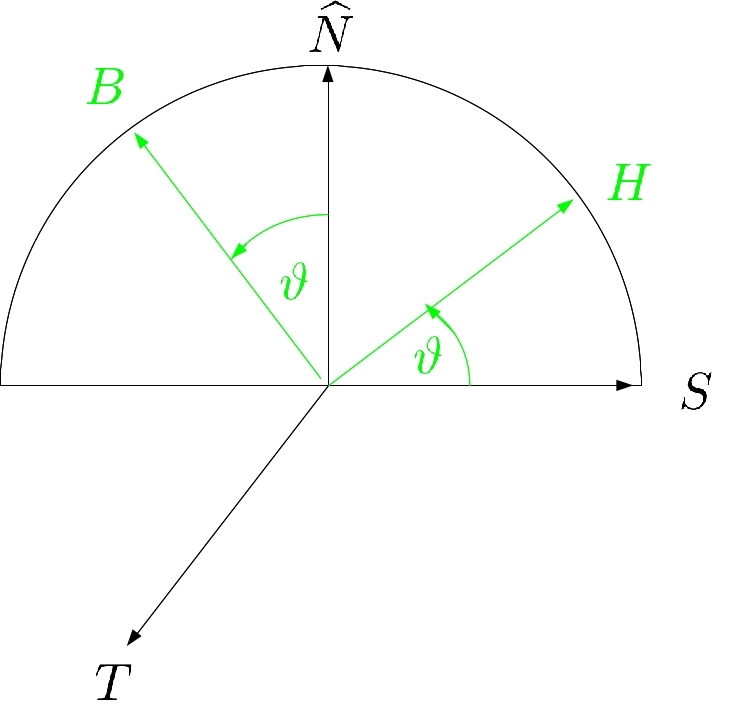
\includegraphics[scale=0.2]{Bilder/Bsp14.jpg} 
\end{center}
\begin{satz}\label{satz243}
 Ist der Winkel \(\vartheta\) zwischen der \uline{Schmiegebene} einer wendepunktfreien \(\C^2\)-Flächenkurve (mit \(\C^1\)-Frenet-Begleitbasis) und der \uline{Tangentialebene} der Fläche, so gewählt, dass gilt
 \begin{align*}
  \begin{matrix}
  H &= \cos \vartheta S + \sin \vartheta \widehat N \\
  B &= -\sin \vartheta S + \cos \vartheta \widehat N
  \end{matrix}
  \quad\text{ bzw. }\quad
  \begin{matrix}
   S &= \cos \vartheta H - \sin \vartheta B \\
   \widehat N &= \sin \vartheta H + \cos \vartheta B
  \end{matrix}
  \quad \text{ (Zurückdrehen!)}
 \end{align*}
 so folgt für die Streifeninvarianten sowie Krümmung und Torsion der Kurve
 \begin{align*}
  &\begin{rcase}
   (1)\quad &\kappa_g = \kappa \cos \vartheta \\
   (2)\quad &\kappa_n = \kappa \sin \vartheta
  \end{rcase}
  \text{ also } \kappa = \sqrt{\kappa_g^2 + \kappa_n^2} \\
  &\;\,(3) \quad \tau_g = \tau - \vartheta' 
 \end{align*}
\end{satz}

\begin{beweis}[von Satz \ref{satz243}]
 \begin{align*}
  T' &= \kappa \cdot H \stackrel{!}{=} = \kappa_g S + \kappa_n \widehat N \Rightarrow (1), (2) \\
  \tau_g &= \langle S', \widehat N \rangle = \langle -(\underbrace{\sin \vartheta H + \cos \vartheta B}_{\widehat N}) \vartheta' + \underbrace{\cos \vartheta (\cancel{-\kappa T} + \tau B) + \sin \vartheta \tau H}_{\tau \cdot \widehat N}, \widehat N \rangle = -\vartheta' + \tau
 \end{align*}
\end{beweis}

\begin{bemerkung}
 \uline{Geraden} (\(T' \equiv 0\)) auf einer Fläche (passen nicht ins Schema) sind sowohl \uline{Geodätische} als auch \uline{Asymptotenlinien} (\(\kappa_g = \kappa_n \equiv 0\))
\end{bemerkung}

\begin{folgerung}
 Für wendepunktfreie Flächenkurven gilt
 \begin{enumerate}
  \item[a)] \uline{Geodätische} sind durch \(\uline{\cos \vartheta = 0}\) bzw. \(\uline{H = \pm \widehat N}\) gekennzeichnet. Der ``Krümmungsvektor'' \(c'' = \kappa \cdot H\) ist stets orthogonal zur Fläche. Schmiegebene und Tangentenebene schneiden sich rechtwinklig.
  \item[b)] \uline{Asymptotenlinien} sind durch \(\uline{\sin \vartheta = 0}\) bzw. \(\uline{B = \pm \widehat N}\) gekennzeichnet. Schmiegebene und Tangentialebene stimmen (bis au die Orientierung) überein. (Deswegen auch ``Schmieglinien'')
 \end{enumerate}
\end{folgerung}

Eine weitere Interpretation von \(\kappa_n\) und \(\tau_g\)

\begin{satz}\label{satz244}
 Für \(\C^2\)-Flächenkurven gilt
 \begin{enumerate}
  \item[a)] In einem Flächenpunkt \(c(s)\) ist \(|\kappa_n(s)|\) die Krümmung und \(\tau_g(s)\) die Torsion derjenigen Geodätischen, die dort die Kurve berührt.
  \item[b)] [Satz von \textsc{Meusnier}] \\
  In einem Kurvenpunkt \(c(s)\) ist \(|\kappa_n(s)|\) die Krümmung des ebenen Normalschnitts der Fläche, die dort die Kurve berührt.
 \end{enumerate}
\end{satz}

\begin{beweis}[von Satz \ref{satz244}] \(\)
 \begin{enumerate}  
  \item[a)] Für Kurve \(c\) und Geodätische \(\widetilde c\) folgt aus \(T = \widetilde T\) auch \[\kappa_n = \widetilde \kappa_n, \, \tau_g = \widetilde \tau_g\]. Wegen \(\widetilde \kappa_g = 0\) (\(\Rightarrow \widetilde \kappa = |\widetilde \kappa_n|, \, \widetilde \vartheta = \const\)) erhält man \[|\kappa_n| = |\widetilde \kappa_n| = \widetilde\kappa, \, \tau_g = \widetilde \tau_g = \widetilde \tau\].
  \item[b)] Für den ebenen Normalschnitt \(\widetilde c\) gilt 
   \begin{align*}
    &\widetilde B \perp \widehat N, \text{ also } \cos \widetilde \vartheta = \left\langle \widetilde B, \widehat N \right\rangle = 0, \\
    &\text{also ebenfalls } |\kappa_n| = |\widetilde \kappa_n | = \widetilde \kappa
   \end{align*}
   \end{enumerate}
  \end{beweis}
 

\begin{folgerung}
 Geodätische auf einer Fläche besitzen in jedem Kurvenpunkt \uline{minimale Krümmung} \(\kappa\) im Vergleich zu allen anderen Flächenkurven durch diesen Punkt mit gleicher Tangentialrichtung.
\end{folgerung}

\begin{beweis}[der Folgerung]
 Für Geodätische \(c\) und Vergleichskurve \(\widetilde c\) gilt
 \[
  \kappa = |\kappa_n | = |\widetilde \kappa_n | \le \sqrt{\kappa_g^2 + \kappa_n^2} = \widetilde \kappa
 \]
\end{beweis}

Wir untersuchen jetzt \(\kappa_n\) und \(\tau_g\) in Abhängigkeit von der Tangentenrichtung in einem festen Kurvenpunkt. \\ Referenzsystem: Hauptkrümmungsrichtungen

\begin{satz}\label{satz245}
 In einem Flächenpunkt sei die Tangentialrichtung \(\uline{T = \cos \varphi Y_1 + \sin \varphi Y_2}\) mit (orthonormierten) Hauptkrümmungsrichtungen \(Y_1, Y_2\) gegeben. Dann gilt
 \begin{align*}
  &\uline{\kappa_n(\varphi) = \kappa_1 \cos^2 \varphi + \kappa_2 \sin^2 \varphi} = H - \sqrt{H^2-K} \cos 2\varphi &\text{[\textsc{euler}sche Formel]}\\
  &\uline{\tau_g (\varphi) = (\kappa_2 - \kappa_1) \sin \varphi \cos \varphi} = + \sqrt{H^2 - K} \sin 2 \varphi
 \end{align*}
\end{satz}

\begin{beweis}[von Satz \ref{satz245}]
 Wegen
 \[
  S = - \sin \varphi Y_1 + \cos \varphi Y_2, \, A(T) = \kappa_1 \cos \varphi Y_1 + \kappa_2 \sin \varphi Y_2
 \]
 ist
 \begin{align*}
  &\kappa_n(\varphi) = \left\langle A(T), T \right\rangle = \kappa_1 \cos^2 \varphi + \kappa_2 \sin^2 \varphi \\
  &\tau_g(\varphi) = \langle A(T), S \rangle = (\kappa_2 - \kappa_1) \sin \varphi \cos \varphi
 \end{align*}
 Aus 
 \begin{align*}
  &H = \frac12 (\kappa_1 + \kappa_2), \, K = \kappa_1 \kappa_2 \Rightarrow \sqrt{H^2 - K} = \frac12 (\kappa_2 - \kappa_1) &[\text{wenn }\kappa_1 \le \kappa_2] \text{ und} \\
  & \cos^2 \varphi - \sin^2 \varphi = \cos 2\varphi, \, 2 \sin \varphi \cos \varphi = \sin 2 \varphi
 \end{align*}
 folgt die zweite Darstellung.
\end{beweis}

\begin{folgerung} \(\)
 \begin{enumerate}
  \item[a)] In einem Flächenpunkt sind die Hauptkrümmungen \(\kappa_1, \kappa_2\) die \uline{Extremalwerte} der Normalkrümmung \(\kappa_n\) bezüglich aller Tangentenrichtungen.
  \item[b)] Trägt man in einem Flächenpunkt in jede Tangentialrichtung die Größe \(\frac{1}{\sqrt{|\kappa_n(\varphi)|}}\) ab, so erhält man die Dupinsche Indikatrix.
 \end{enumerate}
\end{folgerung}

\begin{beweis}[der Folgerung] \(\)
 \begin{enumerate}
  \item[a)] \mat{\frac{\dd}{\dd \varphi} \kappa_n(\varphi) = (\kappa_2 - \kappa_1) \sin \varphi \cos \varphi = 0 \stackrel{\kappa_1 \ne \kappa_2}{\Leftrightarrow} \sin \varphi = 0 \lor \cos \varphi = 0}
  \item[b)] Für \mat{X := \frac{1}{\sqrt{|\kappa_n(\varphi)|}} \cdot T} gilt
  \[
   \Rom2(X,X) = \frac{1}{| \kappa_n(\varphi)|} \Rom2(T,T) = \frac{1}{|\kappa_n(\varphi)|} \underbrace{\langle A(T), T) \rangle}_{\kappa_n(\varphi)} = \pm 1
  \]
 \end{enumerate}

\end{beweis}

\begin{anwendung}
 Auf einer Kugel ist jede Richtung eine Hauptkrümmungsrichtung (nur Nabelpunkte!). Also ist jede sphärische Kurve eine Krümmungslinie mit \(\tau_g \equiv 0\). Weiter ist \(\kappa_n = \kappa_1 \cos^2 \varphi + \kappa_2  \sin^2 \varphi = \kappa_1 = \kappa_2 = \frac{1}{r} = \const.\) (wenn \(r\) der Kugelradius ist). Also gilt
 \begin{align*}
  &\begin{Bmatrix}
   \kappa \sin \vartheta = \frac1r \\
   \tau = \vartheta'
  \end{Bmatrix} 
 \Leftrightarrow
 \begin{Bmatrix}
  \varrho = r \sin \vartheta \\
  \tau = \vartheta'
 \end{Bmatrix}
 \Leftrightarrow
 \begin{Bmatrix}
  \varrho = r \cos \lambda \\
  \tau = - \lambda'
 \end{Bmatrix}
 &\text{ mit } \lambda = \frac{\pi}{2} - \vartheta
 \end{align*}
\end{anwendung}

\subsection{Spezielle Parameter}
Auf einer Fläche gibt es zwar keine BLP wie bei Kurven aber doch einige nützliche spezielle Parameter, z.B. \\ \uline{Krümmungslinienparameter}\index{Krümmungslinienparameter}  
\begin{itemize}
 \item[\(\Leftrightarrow\)] alle Parameterlinien sind Krümmungslinien 
 \item[\(\Leftrightarrow\)] \(x_\varrho \parallel Y_\varrho \, (\varrho = 1,2)\) mit Hauptkrümmungsrichtungen \(Y_1, Y_2\)
\end{itemize}
\uline{Asymptotenlinienparameter}\index{Asymptotenlinienparameter} (existieren nur auf hyperpolischen Flächen, evtl. mit Flachpunkten)
\begin{itemize}
 \item[\(\Leftrightarrow\)] alle Parameterlinien sind Asymptotenlinien
 \item[\(\Leftrightarrow\)] \(x_\varrho \parallel Z_\varrho \, (\varrho = 1,2)\) mit Asymptotenrichtungen \(Z_1, Z_2\)
\end{itemize}

Wie erkennt man solche Parameter?

\begin{satz}\label{satz246} \(\)
 \begin{enumerate}
  \item[a)] Auf einer \uline{nabelpunktfreien} \(\C^2\)-Fläche in der Parameterdarstellung \(u \mapsto x(u)\) sind die Parameterlinien genau dann \uline{Krümmungslinien}, wenn gilt
  \[
   g_{12} = b_{12} = 0
  \]
  In diesem Fall sind die Hauptkrümmungen
  \[
   \kappa_1 = \frac{b_{11}}{g_{11}}, \kappa_2 = \frac{b_{22}}{g_{22}}
  \]
  und die Weingartenschen Ableitungsgleichungen lauten
  \[
   \partial_\varrho N = - \kappa_\varrho x_\varrho \quad (\varrho = 1,2) \qquad [\text{Formel von \textsc{Rodriguez}}]
  \]
  \item[b)] Auf einer rein \uline{hyperbolischen} \(\C^2\)-Fläche sind die Parameterlinien genau dann \uline{Asymptotenlinien}, wenn gilt
  \[
   b_{11} = b_{22} = 0
  \]
 \end{enumerate}
\end{satz}

\begin{beweis}[von Satz \ref{satz246}] \(\)
 \begin{enumerate}
  \item[a)] ``\(\Rightarrow\)'' in Krümmungslinienparametern folgt aus \(x_\varrho \parallel Y_\varrho \, (\varrho = 1,2)\)
  \[
   - \partial_\varrho N = A(x_\varrho) = \kappa_\varrho x_\varrho, \text{ also } (\wein \mu \sigma) = \begin{pmatrix}
                                                                                                       \kappa_1 & 0 \\
                                                                                                       0 & \kappa_2
                                                                                                      \end{pmatrix}
  \]
  und wegen \(\kappa_1 \ne \kappa_2\) (Nabelpunktfreiheit) auch
  \[
   \langle x_1, x_2 \rangle = g_{12} = 0
  \]
  Also ist 
  \[
   (b_{\varrho \sigma} = (g_{\varrho \sigma}) \cdot (\wein \mu \sigma) = \begin{pmatrix}
                                                                          g_{11} \kappa_1 & 0 \\
                                                                          0 & g_{22} \kappa_2
                                                                         \end{pmatrix}
                                                                         = \begin{pmatrix}
                                                                            b_{11} & 0 \\
                                                                            0 & b_{22}
                                                                           \end{pmatrix}
  \]
  ``\(\Leftrightarrow\)'' \(g_{12} = b_{12} = 0 \Rightarrow \wein12 = \wein21 = 0\), d.h. \((\wein \mu \sigma)\) ist Diagonalmatrix. Die Basisvektoren \(x_1, x_2\) sind also Eigenvektoren und definieren die Hauptkrümmungsrichtungen.
  \item[b)]
  \(x_1, x_2\) Asymptotenrichtungen \(\Leftrightarrow \Rom2 (x_1, x_1) = b_{11} = 0 \land \Rom2 (x_2, x_2) = b_{22} = 0\)
 \end{enumerate}

\end{beweis}

\begin{bemerkung}
 Auf einer Kugel und in der Ebene ist jede Parametrisierung eine ``Krümmungslinienparametrisierung'' (\uline{nur Nabelpunkte}) : Jede Richtung ist Hauptkrümmungsrichtung. \\
 In isolierten Nabelpunkten können Singularitäten des Krümmungsliniennetzes auftreten.
 \begin{bsp}
  Ellipsoid
 \end{bsp}
\end{bemerkung}

\begin{bsp} \(\)
 \begin{enumerate}
  \item Auf einer \uline{Rotationsfläche} sind Meridiane und Breitenkreise \uline{ebene Krümmungslinien} (\(g_{12} = b_{12} = 0\))
  \item Auf einer \uline{Wendelfläche} (siehe \(\widehat x\) in Übung 2.1) sind die auf ihr liegenden Geraden und Schraubenlinien \uline{Asymptotenlinien} (\(b_{11} = b_{22} = 0\))
 \end{enumerate}

\end{bsp}

Zur Existenz solcher parameter: Dazu eine Verallgemeinerung des Problems. \par
\uline{Gegeben} seien auf einer \(\C^2\)-Fläche \(u \mapsto x(u)\) zwei linear unabhängige tangentiale \(\C^1\)-Vektorfelder
\begin{align*}
 &u \mapsto X_1(u) = \sum \xi^\mu_1 x_\mu (u) \\
 &u \mapsto X_2(u) = \sum \xi^\mu_2 x_\mu (u)
\end{align*}
\uline{Gesucht} ist eine Parametertransformation \(u \mapsto \overline u = \Phi(u)\), sodass nach der Transformation für \(\overline x = x \circ \Phi^{-1}\) gilt
\[
 \forall_u \overline x_\varrho \big(\Phi(u)\big) \parallel X_\varrho (u)
\]

\uline{Lösung}: Wegen \(x = \overline x \circ \Phi\), also \( x_\mu = \sum \overline x_\sigma \partial_\mu \Phi^\sigma\), d.h.
\begin{align*}
 X_\varrho = \sum \xi^\mu_\varrho x_\mu = \sum \xi^\mu_\varrho \partial \mu \Phi^\sigma \overline x_\sigma \parallel \overline x_\varrho \quad (\varrho = 1,2)
\end{align*}
muss gelten
\begin{align*}
  &\sum \xi^\mu_2 \partial_\mu \Phi^1 = \uline{\xi^1_2 \partial_1 \Phi^1 + \xi^2_2 \partial_2 \Phi^1 = 0} \tag{\(\varrho = 2\)} \\
  &\sum \xi^\mu_1 \partial_\mu \Phi^2 = \uline{\xi^1_1 \partial_1 \Phi^2 + \xi^2_1 \partial_2 \Phi^2 = 0} \tag{\(\varrho = 1\)} 
\end{align*}
Für die Komponententen \(F = \Phi^1, \Phi^2\) von \(\Phi\) müssen also partielle Differentialgleichungen der Form
\begin{align*}
 &a \cdot \partial_1 F + b \cdot \partial_2 F = 0 &\text{bzw.} \\
 &\grad F \parallel \vxy {-b}{a} =: f
\end{align*}
Solche Differentialgleichungen lassen sich in der \uline{Ebene} (bei zwei Parametern) mit einem geeigneten \uline{integrierenden Faktor} \((u^1, u^2) \mapsto \mu(u^1, u^2) \ne 0\) lokal stets lösen: Es existiert eine Funktion \(F\) mit 
\[
 \grad F = \mu \cdot f
\]
(siehe Differentialgleichungen, Stichwort: ``Exakte Differentialgleichungen'') \par
\uline{Problem} dabei: Diese Lösungen sind im Allgemeinen nur \(\C^1\)-differenzierbar (\(a,b \; \C^1\), aber \(\mu \; \C^0 \Rightarrow F \; \C^1\)) und liefern eine nicht zulässige \(\C^1\)-Parametertransformation \(u \mapsto \Phi(u)\) auf der \(\C^2\)-Fläche mit den gewünschten Eigenschaften \(\overline x_\varrho \big(\Phi(u)\big) \parallel X_\varrho(u)\). \par

Anwendung auf Hauptkrümmungsrichtungen bzw. Asymptotenrichtungen:\\
Hier sind erst bei \(\C^3\)-Flächen 2. Grundform und Weingartenmatrix \(\C^1\)-Differenzierbar und damit auch die Hauptkrümmungsrichtungen bzw. Asymptotenrichtungen. Dies liefert

\begin{satz}\label{satz247} \(\)
 \begin{enumerate}
  \item[a)] In der Umgebung eines \uline{Nicht-Nabelpunktes} einer \(\C^3\)-Fläche existiert ein \(\C^1\)-Parameternetz aus \uline{Krümmungslinien}.  
  \item[b)] In der Umgebung eines \uline{hyperbolsichen Punktes}  einer \(\C^3\)-Fläche existiert ein \(\C^1\)-Parameternetz aus \uline{Asymptotenlinien}.
 \end{enumerate}

\end{satz}

\begin{bemerkung} \(\)
 \begin{enumerate}
  \item Erst auf einer \(\C^4\)-Fläche existiert im Allgemeinen eine lokale Krümmungslinien-/Asymptoten\-linien-Parametrisierung, mit der sich vernünftig arbeiten lässt.
  \item Der Satz gilt \uline{nicht} ür höher-dimensionale Hyperflächen.
  \item Ist das Parametergebiet der Fläche \uline{einfach zusammenhängend} (``ohne Löcher''), so exsitert sogar eine globale Transformation auf Krümmungslinien-/Asymptotenlinien-Parametern (falls keine Nabelpunkte stören).
 \end{enumerate}

\end{bemerkung}

\uline{Ergänzung}: Weitere ausgezeichnete, lokal in jedem Punkt existierende Parameter sind:
\begin{enumerate}
 \item[a)] \uline{Geodätische Parallelkoordinaten} bezüglich einer Flächenkurve \(c\) \\
 \;\uline{Erkennungszeichen}: 
 \begin{align*}
  &\big(g_{\varrho \sigma}(u,v)\big) = \begin{pmatrix}
                                      1 & 0 \\
                                      0 & g(u,v)
                                     \end{pmatrix}&\text{falls Geodätische in BLP} \\
  &\big(g_{\varrho \sigma}(u,v)\big) = \begin{pmatrix}
                                        \lambda(u) & 0 \\
                                        0 & \mu(u,v)
                                       \end{pmatrix}&\text{sonst}
 \end{align*}
 \begin{bsp}
  Rotationsfläche mit \(\big(g_{\varrho \sigma}(u,v)\big) = \begin{pmatrix}
                                                             w(u) & 0 \\
                                                             0 & r(u)
                                                            \end{pmatrix}\)
 \end{bsp}
 \item[b)] \uline{Geodätische Polarkoodinaten} (\(c \equiv x_0\)) \\
 \uline{Kennzeichen}: wie unter a)
\end{enumerate}

\section{Vertauschbarkeitsrelationen, BONNETscher Fundamentalsatz}
Die Koeffizienten der Ableitungsgleichungen einer \uline{\(\C^3\)-Hyperfläche im \(\IR^n\)}
\begin{align*}
 \partial_\sigma x_\varrho &= \sum \christ \varrho \mu \sigma x_\mu + b_{\varrho \sigma} N \\
 \partial_\sigma N &= -\sum \wein \mu \sigma x_\mu
\end{align*}
lassen sich alle aus den beiden Grundform-Matrizen berechnen.
\begin{align*}
 &(g_{\varrho \sigma}) \to \left(\christ \varrho \mu \sigma \right) \\
 &(g_{\varrho \sigma}) \text{ und } (b_{\varrho \sigma}) \to \left(\wein \mu \sigma\right)
\end{align*}
Aber sie sind nicht unabhängig voneinander. Die \uline{Vertauschbarkeitsrelationen}\index{Vertauschbarkeitsrelationen}
\begin{align*}
 &\partial_\tau \partial_\sigma x_\varrho = \partial_\sigma \partial_\tau x_\varrho & \partial_\tau \partial_\sigma N = \partial_\sigma \partial_\tau N
\end{align*}
liefern komplizierte differentielle Relationen zwischen ihnen. \par
Zunächst: Hilfsmittel zu ihrer invarianten Beschreibung:
\subsection{Der Riemannsche Krümmungstensor}\index{Riemannscher Krümmungstensor}
Bei einer \(\C^3\)-Fläche sind die zweiten \uline{gewöhnlichen} partiellen Ableitungen der tangentialen Basisfelder \(u \mapsto x_1(u), \dots, x_{n-1} (u)\) vertauschbar. Dies gilt im Allgemeinen \uline{nicht} für die zweiten \uline{kovarianten} partiellen Ableitungen, wenn die Fläche ``krumm''ist, also \(\nabla \ne \dd\) ist. Man erhält
\begin{align*}
 \nabla_\tau \nabla_\sigma x_\varrho - \nabla_\sigma \nabla_\tau x_\varrho = \sum \riem \varrho \mu \sigma \tau x_\mu
\end{align*}
mit Koeffizientenfunktion \(u \mapsto \riem \varrho \mu \sigma \tau (u)\). \par
Wegen
\begin{align*}
 \nabla_{\tau} \nabla_\sigma x_\varrho &= \nabla_\tau \left( \sum \christ \varrho \mu \sigma x_\mu \right) = \sum \partial_\tau \christ \varrho \mu \sigma x_\mu + \sum \christ \varrho {\cancelto{\alpha}{\mu}} \sigma \nabla_\tau x_{\cancelto{\alpha}{\mu}} \\
 &=\sum \left(\partial_\tau \christ \varrho \mu \sigma + \christ \varrho \alpha \sigma \christ \alpha \mu \tau \right) x_\mu
\end{align*}
gilt
\[
 \riem \varrho \mu \sigma \tau = \left(\partial_\tau \christ \varrho \mu \sigma + \christ \varrho \alpha \sigma \christ \alpha \mu \tau \right) - \left(\partial_\sigma \christ \varrho \mu \tau + \christ \varrho \alpha \tau \christ \alpha \mu \sigma \right)
\]
Die Koeffizienten sind offensichtlich \uline{innergeometrisch}. \par
Durch lineare Fortsetzung auf beliebige tangentiale Vektorfelder \(x = \sum X^\varrho x_\varrho, \, Y = \sum Y^\sigma x_\sigma, \, Z = \sum Z^\tau x_\tau\) mittels
\begin{align*}
 R(Y,Z)X := \sum \riem \varrho \mu \sigma \tau X^\varrho Y^\sigma Z^\tau x_\mu
\end{align*}
wird in jedem Flächenpunkt eine dreifach lineare Abbildung 
\[
 R_u \colon (T_u x)^3 \to T_u x
\]
definiert. Das Feld \(u \mapsto R_u\) ist unabhängig von der Ausgangsparametrisierung (siehe später) und nennt es \uline{Riemannsches Krümmungstensorfeld}\index{Riemannsches Krümmungstensorfeld}.

\begin{bemerkung}
 Die Parameterunabhängigkeit sieht man auch an der Darstellung
 \begin{align*}
  R(Y,Z)X = \nabla_Z \nabla_Y X - \nabla_Y \nabla_Z X - \nabla_{[Y,Z]} X
 \end{align*}

\end{bemerkung}

Verwendet wird dabei die durch \([Y,Z] := \dd_Z Y - \dd_Y Z\) definierte \uline{Lie-Klammer}\index{Lie-Klammer} (auch \uline{Kommutator}\index{Kommutator} von \(Y,Z\) genannt), welche zwei tangentialen Vektorfeldern \(Y,Z\) wieder ein tangentiales Vektorfeld \([Y,Z]\) zuordnet (ohne Beweis). \par

Speziell für natürliche Basisfelder \(X = x_\varrho, \, Y = x_\sigma, \, Z = x_\tau\) gilt
\begin{align*}
[x_\sigma, x_\tau] = \partial_\tau x_\sigma - \partial_\sigma x_\tau = 0 
\end{align*}
d.h. sie ``kommutieren'' und es folgt
\begin{align*}
 R(x_\sigma, x_\tau) x_\varrho = \nabla_\tau \nabla_\sigma x_\varrho - \nabla_\sigma \nabla_\tau x_\varrho = \sum \riem \varrho \mu \sigma \tau x_\mu
\end{align*}

\uline{Hinweis}: Oft wird auch die Definition
\begin{align*}
 [Y,Z] = \dd_Y Z - \dd_Z Y, \, T(Y,Z)X = \nabla_Y \nabla_Z X - \dots
\end{align*}
verwendet; ändert nur das Vorzeichen. \par

Zur Bezeichnung ``\uline{Krümmungstensor}'': \\
Eine Ableitung kann als infinitesimale Parallelverschiebung gedeutet werden. \\
Au ``flachen'' Flächen mit \(\nabla = \dd\) gilt \(R \equiv 0\). Infinitesimale durch \uline{gewöhnliche} Parallelverschiebung entstandene Parallelogramme ``schließen sich''. Dies gilt nicht auf ``krummen'' Flächen mit \(\nabla \ne \dd\) bei Verwendung der geodätischen Parallelverschiebung.

\subsection{Weitere kovariante Ableitungen}
Ziel: Fortsetzung der kovarianten Ableitung \(\nabla X\) für Vektorfelder \(X\) auf andere ``Tensorfelder'', z. B. Felder von Bilinearformen (\(\Rom1, \Rom2\)) und von linearen Abbildungen (\(A\)). \par
Trick: Forderung der Gültigkeit der \uline{Produktregel}.

\begin{enumerate}
 \item Wir definieren \(\nabla_\tau \Rom2\) (soll wieder Bilinearform sein) durch
 \begin{align*}
  (\nabla_\tau \Rom2)(x_\varrho, x_\sigma) &:= \partial_\tau \left[\Rom2(x_\varrho, x_\sigma)\right] - \Rom2 (\underbrace{\nabla_\tau x_\varrho}_{\sum \christ \varrho \alpha \tau x_\alpha}, x_\sigma) - \Rom2 (x_\varrho, \underbrace{\nabla_\tau x_\sigma}_{\sum \christ \sigma \alpha \tau x_\alpha}) \\
  &= \partial_\tau b_{\varrho \sigma} - \sum b_{\alpha \sigma} \christ \varrho \alpha \tau - \sum b_{\varrho \alpha} \christ \sigma \alpha \tau =: \nabla_\tau b_{\varrho \sigma}
 \end{align*}
 Für die lineare Fortsetzung
 \[
  (\nabla_Z \Rom2)(X,Y) = \sum \nabla_\tau b_{\varrho \sigma} X^\varrho Y^\sigma Z^\tau
 \]
 auf beliebige tangentiale Vektorfelder \(X,Y,Z\) reduziert man nach
 \begin{align*}
  (\nabla_Z \Rom2)(X,Y) = \dd_Z \left[ \Rom2(X,Y)\right] - \Rom2(\nabla_Z X,Y) - \Rom2(X , \nabla_Z Y)
 \end{align*}
 was die Parameterunabhängigkeit zeigt.

 \begin{bemerkung}
  Anwendung dieses Verfahrens auf die 1. Grundform \(\Rom1\) liefert
  \begin{align*}
   &(\nabla_\tau \Rom1) (x_\varrho, x_\sigma) = \partial_\tau g_{\varrho \sigma} - \gamma_{\varrho \sigma \tau} - \gamma_{\sigma \varrho \tau} \equiv 0 &\text{(siehe Satz \ref{satz215})}
  \end{align*}
   und beweist das \uline{\textsc{Ricci}-Lemma} \(\boxed{\nabla \Rom1 \equiv 0}\)
  \end{bemerkung}
 \item Analog definieren wir \(\nabla_\tau A\) (soll wieder lineare Abbildung sein) durch
 \begin{align*}
  (\nabla_\tau A) (x_\sigma) &:= \nabla_\tau \left[A(x_\sigma)\right] - A(\nabla_\tau x_\sigma) \\
  &= \nabla_\tau \left(\sum \wein \mu \sigma x_\mu \right) - A\left(\sum \christ \sigma \alpha \tau x_\alpha \right) \\
  &= \sum \left(\partial_\tau \wein \mu \sigma \right) + \sum \wein {\cancelto{\alpha}{\mu}} \sigma \nabla_\tau x_{\cancelto{\alpha}{\mu}} \quad- \sum \christ \sigma \alpha \tau A(x_\alpha) \\
  &= \partial_\tau \wein \mu \sigma x_\mu + \sum \wein \alpha \sigma \christ \alpha \mu \tau x_\mu - \sum \wein \mu \alpha \christ \sigma \alpha \tau x_\mu \\
  &= \left[\partial_\tau \wein \mu \sigma + \sum \wein \alpha \sigma \christ \alpha \mu \tau - \sum \wein \mu \alpha \christ \sigma \alpha \tau \right] x_\mu \\
  &=: \left(\nabla_\tau \wein \mu \sigma \right) x_\mu
 \end{align*}
 Für die lineare Fortsetzung
 \[
  \nabla_Z A)(Y) = \sum (\nabla_\tau \wein \mu \sigma) Y^\sigma Z^\tau x_\mu
 \]
 auf beliebige tangentiale Vektorfelder \(Y,Z\) errechnet man wieder 
 \[
  (\nabla_\tau A) (Y) = \nabla_Z \left[A(Y)\right] - A(\nabla_Z Y)
 \]
 was die Parameterunabhängigkeit zeigt.
\end{enumerate}

\subsection{Die Gauß- und Codazzigleichungen}
Wir beschreiben die Vertauschbarkeitsrelationen durch die Operatoren \(R, \nabla \Rom2, \nabla A\).

\subsubsection{1. Die Gaußschen Ableitungsgleichungen}

\begin{align*}
 &\partial_\sigma x_\varrho = \nabla_\sigma x_\varrho + \Rom2(x_\varrho, x_\sigma) N \quad\Rightarrow \\
 &\partial_\tau \partial_\sigma x_\varrho = \nabla_\tau \nabla_\sigma x_\varrho + \Rom2\left( \nabla_\sigma x_\varrho, x_\tau\right) N + \partial_\tau \left[\Rom2(x_\varrho, x_\sigma)\right] N - \Rom2(x_\varrho, x_\sigma) A(x_\tau) \Rightarrow \\
 &0 = (\nabla_\tau \nabla_\sigma x_\varrho - \nabla_\sigma \nabla_\tau x_\varrho) - \big(\Rom2(x_\varrho, \sigma) A(x_\tau) - \Rom2(x_\varrho, x_\tau)A(x_\sigma)\big) \\
 &+[ \cancel{\Rom2 (\nabla_\sigma x_\varrho, x_\tau)} - \xcancel{\Rom2(\nabla_\tau x_\varrho, x_\sigma)} + (\nabla_\tau \Rom2)(x_\varrho, x_\sigma) - (\nabla_\sigma \Rom2)(x_\varrho, x_\tau) \\
 &+ \xcancel{\Rom2( \nabla_\tau x_\varrho, x_\sigma)} - \cancel{\Rom2( \nabla_\sigma x_\varrho, x_\tau)} + \Rom2 (x_\varrho, \underbrace{\nabla_\tau x_\sigma - \nabla_\sigma x_\tau}_{= 0})] N \quad\Leftrightarrow \\
 &\text{(Aufspaltung in Tangential- und Normalanteil)} \\
 &\boxed{R(x_\sigma, x_\tau) x_\varrho = \Rom2 (x_\varrho, x_\sigma) A(x_\tau) - \Rom2(x_\varrho, x_\tau) A(x_\sigma)} \\
 &\boxed{(\nabla_\tau \Rom2)(x_\varrho, x_\sigma) = (\nabla_\sigma \Rom2)(x_\tau)}
\end{align*}

\subsubsection{2. Die Weingartenschen Ableitungsgleichungen}

\begin{align*}
 -\partial_\sigma N &= A(x_\sigma) \\
 -\partial_\tau \partial_\sigma N &= \partial_\tau \left[A(x_\sigma)\right] = \nabla_\tau \left[A(x_\sigma)\right] + \Rom2 \big(A(x_\sigma), x_\tau\big) N \\
 & = (\nabla_\tau A)(x_\sigma) + A(\nabla_\tau x_\sigma) + \big(A(x_\sigma), A(x_\tau)\big) N \quad \Rightarrow \\
 0 &= - (\partial_\tau \partial_\sigma N - \partial_\sigma \partial_\tau N) = (\nabla_\tau A)(x_\sigma) - (\nabla_\sigma A)(x_\tau) + A(\underbrace{\nabla_\tau x_\sigma - \nabla_\sigma x_\tau}_{= 0}) \quad \Leftrightarrow \\
 &\boxed{(\nabla_\tau A)(x_\sigma) = (\nabla_\sigma A)(x_\tau)}
\end{align*}

Lineare Fortsetzung liefert

\begin{satz}\label{satz251}
 Die Vertauschbarkeitsrelationen der Gaußschen Ableitungsgleichungen einer \(\C^3\)-Hyperfläche im \(\IR^n\) lauten parameterunabhängig
 \begin{align*}
  &\boxed{R(Y,Z)X = \Rom2 (X,Y) A(Z) - \Rom2 (X,Z) A(Y)} &\text{Gaußgleichung} \tag 1 \\
  &\boxed{(\nabla_Z \Rom2)(X,Y) = (\nabla_Y \Rom2)(X,Z)} &\text{Codazzigleichung für } \Rom2 \tag 2
 \end{align*}
 Die Vertauschbarkeitsrelationen der Weingartenschen Ableitungsgleichungen lauten parameterunabhängig
 \begin{align*}
  &\boxed{(\nabla_Z A)(Y) = (\nabla_Y A)(Z)} &\text{Codazzigleichung für } A \tag 3 
 \end{align*}
 und sind äquivalent zur Codazzigleichung für \(\Rom2\).
\end{satz}

\begin{beweis}[der Äquivalenz (2) \(\Leftrightarrow\) (3) von Satz \ref{satz251}]
 Für alle \(X,Y\) gilt
 \begin{align*}
  \Rom2(X,Y) &= \Rom1 \big(A(X), Y\big) = \Rom1\big(X, A(Y)\big) \quad \Rightarrow \\
  (\nabla_Z \Rom2) (X,Y) &= \dd_z[\Rom2(X,Y)] - \Rom2 (\nabla_Z X, Y) - \Rom2 (X, \nabla_Z Y) \\
  &=\dd_Z [\Rom1 (X,A(Y))] - \Rom1 \big(\nabla_Z X, A(Y)\big) - \Rom1 \big(X, A(\nabla_Z Y)\big) \\
  &\quad- \underbrace{\Rom1 \big(X, \nabla_Z [A(Y)]\big) + \Rom1 \big(X,\nabla_Z [A(Y)]\big)}_{= 0} \\
  &= \underbrace{(\nabla_Z \Rom1)}_{= 0}\big(X, A(Y)\big) + \Rom1 \big( X, \nabla_Z [A(Y)] - A(\nabla_Z Y) \big) \\
  &= \Rom1 \big(X, (\nabla_Z )(Y) \big)
 \end{align*}
 Also ist (2) äquivalent zu
 \begin{align*}
  \Rom1 \big(X, (\nabla_Z A)(Y) - (\nabla_Y A)(Z) \big) = 0 \text{ für alle }X
 \end{align*}
 also äquivalent zu (3).
\end{beweis}

\begin{bemerkung}
 Gleichung (1) beweist (nochmal) die Parameterunabhängigkeit und Linearität des Krümmungs\-tensors.
\end{bemerkung}
\setcounter{korollar}{1}
\begin{korollar}\label{korollar252}
 Bezüglich einer Parametrisierung \(u \mapsto x(u)\) einer \(\C^3\)-Hyperfläche im \(\IR^n\) lauten die Vertauschbarkeitsrelationen der Abbildungsgleichungen
 \begin{align*}
  &\riem \varrho \mu \sigma \tau = b_{\varrho \sigma} \wein \mu \tau - b_{\varrho \tau} \wein \mu \sigma &\text{(Gaußgleichung)} \tag{1} \\
  &\nabla_\tau b_{\varrho \sigma} = \nabla_\sigma b_{\varrho \tau} &\text{Codazzigleichung für } (b_{\varrho \sigma}) \tag{2} \\
  &\nabla_\tau \wein \mu \sigma = \nabla_\sigma \wein \mu \tau &\text{Codazzigleichung für } (\wein \mu \sigma) \tag{3}
 \end{align*}
\end{korollar}

Definiert man die 4-lineare \uline{Krümmungsform}
\[
 R(Y,Z) (X,W) := \Rom1 \big(R(Y,Z)X, W\big)
\]
in Koordinaten
\[
 \uline{R_{\varrho \nu \,\sigma \tau} = \sum g_{\mu \nu} \riem \varrho \mu \sigma \tau}
\]
so gilt
\begin{align*}
 (1) &\Leftrightarrow R(Y,Z)(X,W) = \Rom2(X,Y) \Rom2(W,Z) - \Rom2(X,Z) \Rom2(W,Y) \\
 &\Leftrightarrow R_{\varrho \nu \,\sigma \tau} = b_{\varrho \sigma} b_{\nu \tau} - b_{\varrho \tau} b_{\nu \sigma} \quad (\ast)
\end{align*}

\begin{folgerung} \(\)
 \begin{enumerate}
  \item Die Krümmungsform ist nicht nur in \((Y,Z)\), sondern auch in \((W,Z)\) \uline{schiefsymmetrisch} \big(Analog für die Indexpaare \((\sigma, \tau)\) und \((\varrho, \nu)\) in \((\ast)\)\big).
  \item Alle \((2 \times 2)\)-Unterdeterminanten der Matrix \((b_{\varrho \sigma})_{\varrho, \sigma = 1, \dots, n-1}\) sind \uline{innergeometrisch} (``Schnittkrümmungen'').
 \end{enumerate}
\end{folgerung}

\subsubsection{Spezialisierung auf 2-Flächen im \(\IR^3\)}
Hier sind in \((\ast)\) nur die Indexpaare \((\varrho, \nu) = (1,2)\) und \((\sigma,\tau) = (1,2)\) wesentlich und man erhält.
\begin{align*}
 (1) \Leftrightarrow R_{12\,12} = b_{11}b_{22}-b_{12}b_{21} = b
\end{align*}
Ebenso folgt aus der Symmetrie von \((b_{\varrho \sigma})\):
\begin{align*}
 (2) \Leftrightarrow \begin{Bmatrix}
                      \nabla_2 b_{11} &= \nabla_1 b_{12} \\
                      \nabla_1 b_{22} &= \nabla_2 b_{12}
                     \end{Bmatrix}
\end{align*}
\setcounter{folgn}{2}
\begin{folgn}
 Speziell für \(\C^3\)-Flächen im \(\IR^3\) ist die Gaußgleichung äquivalent zu
 \begin{align*}
  &\fcolorbox{red}{white}{\(K = \frac{R_{12 \, 12}}{g}\)} &\text{(\uline{Theorema egregium} von Gauß)} \tag {1'} \\
  &\fcolorbox{red}{white}{\(\begin{aligned}
           \nabla_2 b_{11} &= \nabla_1 b_{12} \\
           \nabla_1 b_{22} &= \nabla_2 b_{12}
          \end{aligned}\)} &\text{(\uline{Gleichung von Mainardi-Codazzi})} \tag{2'}
 \end{align*}
 Insbesondere ist die Gaußsche Krümmung eine innergeometrische Größe.
\end{folgn}

\subsection{Der BONNETsche Fundamentalsatz}
Die Ableitungsgleichungen einer Hyperfläche im \(\IR^n\) 
\begin{align*}
 \begin{Bmatrix}
  \partial_\sigma {\color{red}x_\varrho} = \sum {\color{green}\christ \varrho \mu \sigma} {\color{red}x_\mu} + {\color{green}b_{\varrho \sigma}} {\color{red}N} \\
  \partial_\sigma {\color{red}N} = - \sum {\color{green}\wein \mu \sigma} {\color{red}x_\mu}  
 \end{Bmatrix} \tag {\(\ast\)}
\end{align*}
bilden bei {\color{green}bekannten} Funktionen \(u \mapsto \big(g_{\varrho \sigma}(u)\big), \big(b_{\varrho \sigma}(u)\big)\) [\(\to \christ \varrho \mu \sigma (u), \wein \mu \sigma (u)\)], definiert au ein Gebiet \(G \subset R^{n-1}\) ein \uline{System partieller Differentialgleichungen 1. Ordnung} für {\color{red}gesuchte} Abbildungen \(u \mapsto x_\varrho(u), N(u)\). \\
Aus diesen lässt sich die Fläche selbst gewinnen durch Lösen des Systems
\begin{align*}
 \partial_\varrho {\color{red}x} = {\color{green}x_{\varrho}} \tag{\(\ast \ast\)}
\end{align*}
Solche Systeme sind genau dann \uline{lokal eindeutig lösbar}, wenn sogenannte \uline{Integrabilitätsbedingungen} für die Koeffizientenfunktionen erfüllt sind, die man erhält, indem man die Vertauschbarkeitsrelationen (bei \((\ast)\) etwa \(\partial_\tau \partial_\sigma x_\varrho = \partial_\sigma \partial_\tau x_\varrho, \partial_\tau \partial_\sigma N = \partial_\sigma \partial_\tau N\)) formal auswertet.\par
Zuständig ist der \uline{Satz von \textsc{Frobenius}}. \par
Beim System \((\ast)\) sind die Integrabilitätsbedingungen gerade die Gauß- und Codazzigleichungen und beim System \((\ast \ast)\) lauten sie \(\partial_\sigma x_\varrho = \partial_\varrho x_\sigma\) und sind erfüllt, wenn mann in \((\ast) (g_{\varrho \sigma})\) und \((b_{\varrho \sigma})\) [\(\to (\christ \varrho \mu \sigma)\)] als symmetrisch in \((\varrho, \sigma)\) vorausgesetzt. \par
Damit gilt (zunächst für \(n = 3\)):

\setcounter{set}{3}
\begin{satz}\label{satz254}\(\)
 \begin{enumerate}
  \item[a)] Auf einem Gebiet \(G \in \IR^2\) seien
  \begin{itemize}
   \item eine symmetrische positiv definite \(\C^2\)-Matrixfunktion
   \[    u \in G \mapsto \big(\overline g_{\varrho \sigma}(u)\big) \in M(2,2;\IR)
   \]
   \item eine symmetrische \(\C^1\)-Matrixfunktion
   \[
    u \in G \mapsto \big(\overline b_{\varrho \sigma}(u)\big) \in M(2,2;\IR)
   \]
  \end{itemize}
  vorgegeben, welche
  \begin{itemize}
   \item das Theorema egregium (1') \(\overline R_{12 \, 12} = \det (\overline b_{\varrho \sigma})\)
   \item die Mainardi-Codazzi-Gleichung (2') \(\begin{cases}
                                                &\overline \nabla_2 \overline b_{11} = \overline \nabla_1 \overline b_{12} \\
                                                &\overline \nabla_1 \overline b_{22} = \overline \nabla_2 \overline b_{12}
                                               \end{cases}\) 
  \end{itemize}
  formal erfüllen. \par
  Weiter seien ein Parameterwert \(\stackrel \circ u \in G\), ein Punkt \(\stackrel \circ x \in \IR^3\) und zwei Vektoren \(\stackrel \circ x_1, \stackrel \circ x_2\) mit \(\forall_{\varrho, \sigma} \left\langle \stackrel \circ x_\varrho, \stackrel \circ x_\sigma \right\rangle = \overline g_{\varrho \sigma} \left(\stackrel \circ x\right)\)  \(\left( \to N = \frac{\stackrel \circ x_1 \times \stackrel \circ x_2}{\left|\left|\stackrel \circ x_1 \times \stackrel \circ x_2 \right|\right|}\right)\) gegeben. \par
  Dann gibt es \uline{genau eine} \(\C^3\)-Fläche in einer Parameterdarstellung \(x \colon u \in U\left(\stackrel \circ u\right) \subset G \mapsto x(u) \in \IR^3\) mit \(x\left(\stackrel \circ x\right) = \stackrel \circ x, \partial_\varrho x\left(\stackrel \circ u\right) = \stackrel \circ x_\varrho \, (\varrho = 1,2)\) deren Grundformmatrizen \((g_{\varrho \sigma})\) und \((b_{\varrho \sigma})\) gerade die vorgegebenen Matrizen \(\left(\overline g_{\varrho \sigma}\right)\) und \(\left(\overline b_{\varrho \sigma}\right)\) sind.
  \item[b)] Zwei \(\C^3\)-Flächen in Parametrisierungen \(u \mapsto x(u), u \mapsto \widetilde x(u)\) mit gleichen Grundformmatrizen \((g_{\varrho \sigma}) =(\widetilde g_{\varrho \sigma}), (b_{\varrho \sigma}) = (\widetilde b_{\varrho \sigma})\) stimmen überein bis auf eine eigentliche Bewegung des \(\IR^3\), d.h. es gilt
  \[
   \widetilde x = Dx + t \text{ mit } D \in SO(3,\IR) \text{ mit } t \in \IR^3
  \]
 \end{enumerate}
\end{satz}

\begin{beweis}[von Satz \ref{satz254}]
 Wie in der Kurventheorie, unter Verwendung des Satzes von Frobenius statt des entsprechenden Satzes über gewöhnliche Differentialgleichungssystem. \par
 1. und 2. Grundform bilden als ein \uline{vollständiges} System allerdings \uline{nicht unabhängiger} Invarianten für eine Fläche.
\end{beweis}
\subsubsection{Schlussbemerkungen}
\begin{enumerate}
 \item Im Unterschied zur Kurventheorie liefert der \textsc{Bonnet}sche Fundamentalsatz im Allgemeinen nur \uline{lokale} Lösungen (Ist aber das Parametergebiet einfach zusammenhängend, existiert sogar eine globale Lösung).
 \item
\end{enumerate}

{\Huge Hier fehlt noch was}
\begin{beweis}[von Satz \ref{satz261}]
Wir betrachten zunächst \uline{Normalvariationen} mit \(V(u) = f(u) \cdot N(u)\) wobei \(f\) eine \(\C^1\)-Funktion ist. Dann gilt
\begin{align*}
 &V_\sigma = (\partial_\sigma f) N - f \sum \wein \mu \sigma x_\mu \text{ also } \langle V_\sigma, x_\varrho \rangle = -f \sum \wein \mu \sigma g_{\mu \varrho} = -f b_{\varrho \sigma} \\
 &\langle V_\sigma, x_\varrho \rangle + \langle V_\varrho, x_\sigma \rangle = -2 b_{\varrho \sigma} \\
 &\sum_{\varrho, \sigma} g^{\varrho \sigma} \big(\langle V_\sigma, x_\varrho \rangle + \langle V_\varrho, x_\sigma \rangle \big) = -2 f \sum g^{\varrho \sigma} g_{\sigma \varrho} = -2f \sum \wein \varrho \varrho = -4 f \cdot H
\end{align*}

\uline{Ergebnis}:
\begin{align*}
 a'(0) = \frac12 \int\limits_\Omega \frac{1}{\sqrt{g(u)}} g(u) \big(-4 f(u) \cdot H(u)\big) \dd u = -2 \int\limits_\Omega f(u) \cdot H(u) \cdot \underbrace{\sqrt{g(u)} \dd u}_{= \dd A}
\end{align*}
(\uline{1. Normalvariation des Flächeninhalts})\par
Gilt \(a'(0)\) für alle \(\C^1\)-Variationen, insbesondere für alle \(\C^1\)-Normalvariationen, d.h. für alle \(\C^1\)-Funktionen \(f\), so liefert das Fundamentallemma der Variationsrechnung \(\uline{H \equiv 0}\) in \(\Omega\). \par
Lässt man auch einen tangentialanteil im Variationsvektorfeld \(V\) zu, so erhält man nichts Neues:\\
Für \(\overline V = \sum \eta^\mu x_\mu\) gilt
\begin{align*}
 &\overline V_\sigma = \sum \big(\partial_\sigma \eta^\mu + \eta^\alpha \christ \alpha \mu \sigma \big) x_\mu + (\dots) N \\
 \Rightarrow & \langle \overline V_\sigma, x_\varrho \rangle = \sum \big(g_{\mu \varrho} \partial_\sigma \eta^\mu + \eta^\alpha \gamma_{\alpha \varrho \sigma}\big) \\
 \Rightarrow & \langle \overline V_\sigma, x_\varrho \rangle + \langle \overline V_\varrho, x_\sigma \rangle = \sum \big( g_{\mu \varrho} \partial_\sigma \eta^\mu + g_{\mu \sigma} \partial_\varrho \eta^\mu + \eta^\alpha \partial_\alpha g_{\varrho \sigma}\big) \\
 \Rightarrow &\sum_{\varrho, \sigma} g^{\varrho \sigma} \big(\langle \overline V_\sigma, x_\varrho \rangle + \langle \overline V_\varrho, x_\sigma \rangle \big) = \sum \big(\partial_\sigma \eta^\sigma + \partial_\varrho \eta^\varrho + g^{\varrho \sigma} (\partial_\alpha g_{\varrho \sigma}) \eta^{\alpha}\big) \\
 &\stackrel{\text{Hilfssatz}}{=} 2 \sum \left(\partial_\alpha \eta^\alpha + \frac12 \frac{\partial_\alpha g}{g} \eta^\alpha \right) = 2 \sum \left( \partial_\alpha \eta^\alpha + \frac{\partial_\alpha \sqrt{g}}{\sqrt{g}} \eta^\alpha \right) \\
 &= \frac2{\sqrt{g}} \sum \partial_\alpha \left(\sqrt{g} \eta^\alpha \right) = \frac2{\sqrt{g}} \left( \partial_1 (\sqrt{g} \eta^1) + \partial_2(\sqrt{g} \eta^2)\right) \\
\end{align*}
\begin{align*}
 \Rightarrow  \overline a'(0) &= \frac12 \int\limits_\Omega \frac{1}{\sqrt{g(u)}} g(u) \frac{2}{\sqrt{g(u)}} \sum_\alpha \big(\sqrt{g(u)} \eta^\alpha(u)\big) \dd u \\
 &= \int\limits_\Omega \big( \partial_1(\sqrt{g} \eta^1)(u^1, u^2) + \partial_2(\sqrt{g}\eta^2)(u^1,u^2)\big) \dd u^1 \dd u^2
\end{align*}
Ein solches Integral lässt sich nach dem (zweidimensionalen) \uline{Satz von \textsc{Stokes}} in ein Integral über den Rand \(\partial \Omega\) umformen \mat{\left(\int\limits_\Omega \dd \varphi = \int\limits_{\partial\Omega} \varphi\right)}. Beweis nur für den Spezialfall \(\overline \Omega = [a, b] \times [c, d]\):
\begin{align*}
 \overline a'(0) &= \int_c^d \left(\int_a^b \partial_1 (\sqrt{g} \eta^1)(u^1, u^2) \dd u^1\right) \dd u^2 + \int_a^b \left(\int_c^d \partial_2 (\sqrt{g}\eta^2)(u^1, u^2) \dd u^2 \right) \dd u^1 \\
 &= \int_c^d \big( (\sqrt{g}\eta^1)(b, u^2) - (\sqrt{g}\eta^1)(a, u^2)\big)\dd u^2 + \int_a^b \big((\sqrt{g}\eta^2)(u^1, d) - (\sqrt{g}\eta^2)(u^1, c) \big) \dd u^1 \\
 &= 0
\end{align*}
wegen \(\left.\overline V\right|_{\partial \Omega} = 0 \Leftrightarrow \left. \eta^1 \right|_{\partial \Omega} = \left. \eta^2 \right|_{\partial \Omega} = 0\) \par
Man erhält also durch Tangentialanteile in der Variation keine Verschärfung des Satzes.
\end{beweis}

\subsubsection{Wichtig!}
Die Bedingung \(H \equiv 0\) ist nur notwendig für die Minimalität des Flächeninhalts bei fester Randkurve. \\
Mögliche Situationen:
\begin{itemize}
 \item Indefinit stationärer Flächeninalt \(\to\) \uline{Instabile Minimalfläche}
 \item Relatives Minimum \(\to\) \uline{Stabile Minimalfläche}
 \item Absolutes Minimum \(\to\) \uline{Minimierende Minimalfläche}
\end{itemize}

\subsubsection{\uline{Ergänzungen} aus Physik und Analysis}
\begin{enumerate}
 \item \uline{Stabile Minimalflächen} lassen sich durch Seifenhäute realisieren (\textsc{Plateau} 1850). \\
 Geschlossene Raumkurve aus Draht in Seifenlauge bringen. Die eingespannte Haut ist eine Minimalfläche. Physikalischer Hintergrund: Druckdifferenz Außen/Innen ist proportional zu \(H\). Bei Druckausgleich (\(H = 0\)) wird die Oberfläche minimiert.
 \begin{bemerkung}
  Bei geschlossenen ``Seifenblasen'' ist \(\Delta p\) proportional zu \(H = \const. \ne 0\) (\(\to\) cmc-Flächen: ``constant mean currature'')
 \end{bemerkung}
 \item \uline{\textsc{Plateau}sches Problem}: Existiert zu jeder einfach geschlossenen rektifizierbaren Kurve eine eingespannte (stabile) Minimalfläche? \\
 \uline{Antwort}: Es existiert immer eine singularitätenfreie minimierende Lösung. (Teillösungen 1930 (Douglas, Radó), Endgültige Lösung 1970 (Ossermann, Gulliver))
\end{enumerate}

